%%
%% Book containing everything in this repo
%% COMPILE WITH XeLaTeX
%%

\documentclass[
 12pt,                       % Font size
 a4paper                     % Paper type
]{book}

% Packages
\usepackage[
 margin=2.7cm,               % Margin size
 marginparwidth=2cm,         % Margin note size
 marginparsep=3mm,           % Space between margin and text
 headheight=15pt             % Header height (fix that stupid warn from fancyhdr)
]{geometry}
\usepackage[romanian]{babel} % Romanian characters support
\usepackage{indentfirst}     % Add paragraph indentation even after a section
\usepackage{marginnote}      % Notes on the margins of a document (more advanced \marginpar)
\usepackage{titlesec}        % Customize titles
\usepackage{hyperref}        % Hyperlink support
\usepackage{graphicx}        % Image support
\usepackage{xcolor}          % Custom colors
\usepackage{fancyhdr}        % Custom headers
\usepackage{etoolbox}        % Customize chapters
\usepackage[titles]{tocloft} % Customize ToC
\usepackage{blindtext}       % Sample filler text

% Image path
\graphicspath{ {./src/} }

% Hyperlink configuration
\hypersetup{
 colorlinks=true,
 urlcolor=black,
 linkcolor=black  % ToC links color
}

% Colors
\definecolor{gray75}{gray}{0.75}

% Custom format for titles, sections, subsecions etc.
\titleformat{\chapter}[hang]{\Large}{\thechapter\hspace{15pt}\textcolor{gray75}{|}\hspace{15pt}}{0pt}{\Large}
\renewcommand{\thesection}{\arabic{section}}%
\titleformat*{\section}{\large\bfseries}
\titleformat{\subsection}{\normalfont\normalfont\bfseries}{}{1.5em}{}

% Custom commands
% Format: \newcommand{\command}[variable]{action #variable}
\newcommand{\rom}[1]{\uppercase\expandafter{\romannumeral #1\relax}} % Roman numerals
\newcommand{\textbfit}[1]{\textbf{\textit{#1}}}                      % combine bold and italic
\newcommand{\operatitle}{}                                           % to not get errors
\newcommand{\operaauthor}{}                                          % to not get errors

% Customize \marginnote font
\renewcommand\marginfont{\ttfamily\footnotesize}

% Make \ttfamily hyphenate words for the margin notes
\DeclareFontFamily{OT1}{cmtt}{\hyphenchar\font=-1}
\DeclareFontFamily{\encodingdefault}{\ttdefault}{\hyphenchar\font=`\-}
\DeclareFontFamily{T1}{cmtt}{\hyphenchar\font=45}

% ToC customization
\setcounter{tocdepth}{0}     % Make only chapters appear in ToC
\renewcommand{\cftdot}{}     % Remove ToC dots

% Custom fancy styles
\fancypagestyle{chapterfancystyle}{
 \fancyhf{}
 \fancyfoot[LE,RO]{\thepage}
 \renewcommand{\headrulewidth}{0pt}
 \renewcommand{\footrulewidth}{1pt}
}

\fancypagestyle{tocfancystyle}{
 \fancyhf{}
 \fancyhead[LE]{Cuprins}
 \fancyfoot[LE,RO]{\thepage}
 \renewcommand{\headrulewidth}{2pt}
 \renewcommand{\footrulewidth}{1pt}
}

\fancypagestyle{plain}{
 \fancyhf{}
 \fancyhead[LE]{\small\textsc{Esee pentru bacalaureat}}
 \fancyhead[RO]{
  \begingroup
    \small
    \let\textbfit\relax
    \textsc{\operatitle\ -- \operaauthor}
  \endgroup
 }
 \fancyfoot[LE,RO]{\thepage}
 \renewcommand{\headrulewidth}{2pt}
 \renewcommand{\footrulewidth}{1pt}
}

% Patch chapter to use custom header
\patchcmd{\chapter}{\thispagestyle{plain}}{\thispagestyle{chapterfancystyle}}{}{}



%%%%%%%%%%%%%%%%%%



\begin{document}
\pagestyle{empty}
% Create a title page
\begin{titlepage}
 \centering
 \vspace*{1cm}
 \vspace{4\baselineskip}
 {\Huge
 Eseuri pentru bacalaureatul la \\ Limba și Literatura Română\par}
 \vspace{4\baselineskip}
 de\par
 {\Large\textsc{Dobrete Andrei-Robert}\par}
 \vfill
 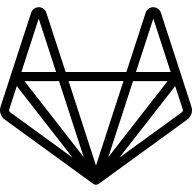
\includegraphics[height=\fontcharht\font`\B]{gitlab}
 \url{gitlab.com/Andy3153/eseuri_bac_romana}\par
 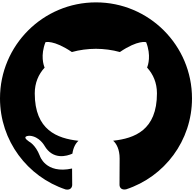
\includegraphics[height=\fontcharht\font`\B]{github}
 \url{github.com/Andy3153/eseuri_bac_romana}\par
 \vspace{1.5\baselineskip}
 {\large\LaTeXe}
\end{titlepage}

% Disable bold in ToC
\addtocontents{toc}{\string\renewcommand{\protect\cftchappagefont}{\protect\normalfont}}
\addtocontents{toc}{\string\renewcommand{\protect\cftchapfont}{\protect\normalfont}}
\addtocontents{toc}{\string\renewcommand{\protect\cftchapleader}{\protect\normalfont\protect\cftdotfill{\protect\cftsecdotsep}}}


\tableofcontents % Generate the ToC

%\addtocontents{toc}{~\hfill\textbf{Pagina}\par} % text above page nr

\pagestyle{plain}


% Beginning of text

% esee
% gen epic
% harap-alb
\chapter{Eseu cu privire la tema și viziunea despre lume dintr-un basm cult studiat}
% Commands
\renewcommand{\operatitle}{\textbfit{„Povestea lui Harap-Alb”}} % title of the text
\renewcommand{\operaauthor}{Ion Creangă} % author of the text


% Beginning of text
\subsection{Context}

\operatitle\ de \operaauthor\ este un basm cult, publicat în revista \textit{„Convorbiri literare”}, în anul 1877.


\section{Evidențierea trăsăturilor care fac posibilă încadrarea basmului studiat în specia literară pe care o ilustrează}
\marginnote{personaje simbolice}[0.3cm]
Basmul cult este o specie narativă pluriepisodică implicând fabulosul, cu numeroase personaje purtătoare ale unor valori simbolice, întruchipând binele și răul în diversele lor ipostaze. Personajele îndeplinesc, prin raportare la protagonist, o serie de funcții (antagonistul, ajutoarele, donatorii), unele având puteri supranaturale.

\marginnote{prezența fabulosului}[0.3cm]
Acțiunea basmului implică prezența fabulosului și este supusă unor stereotipii care înfățișează parcurgerea drumului maturizării de către erou. Conflictul dintre bine și rău se încheie prin victoria forțelor binelui. Reperele temporale și spațiale sunt vagi, nedeterminate. Elemente de compoziție tipice vizează clișee compoziționale/formule specifice, cifre și obiecte magice, procedeul triplicării.


\section{Ilustrarea temei prin episoade/citate/secvențe comentate}
Titlul sugerează tema basmului: maturizarea mezinului craiului. Numele personajului îi reflectă condiția duală: rob, slugă (Harap) de origine nobilă (Alb). Motive narative specifice, prezente și în \operatitle, sunt: superioritatea mezinului, călătoria, supunerea prin vicleșug, muncile, demascarea răufăcătorului (Spânul), pedeapsa, căsătoria.


\section{Prezentarea elementelor de structură și de compoziție ale textului narativ, semnificative pentru tema și viziunea despre lume din basmul cult studiat {\footnotesize\normalfont (de exemplu: acțiune, conflict, relații temporale și spațiale, incipit, final, tehnici narative, perspectivă narativă, registre stilistice, limbajul personajelor etc.)}}
Întâmplările sunt relatate din perspectiva unui narator omniscient, care intervine adesea prin comentarii sau reflecții caracterizate prin umor sau oralitate. Narațiunea la persoana a \rom{3}-a alternează cu dialogul.

Subiectul basmului urmărește modul în care personajul principal, Harap-Alb, parcurge un drum al inițierii, la finalul căruia devine împărat, adică trece într-un plan superior de existență, care înseamnă modificarea statutului social și spiritual al eroului (caracterul de \textit{Bildungsroman} al basmului).

\marginnote{compoziție}[0.8cm]
Cele trei ipostaze ale protagonistului corespund, în plan compozițional, unor părți narative, etape ale drumului inițiatic: etapa inițială, de pregătire pentru drum, la curtea craiului -- \textit{„fiul craiului”, „mezinul”} (naivul); parcurgerea drumului inițiatic -- \textit{Harap-Alb} (novicele/cel supus inițierii); răsplata -- \textit{împăratul} (inițiatul).

\marginnote{tehnică narativă}[0.8cm]
Creangă utilizează triplicarea (triplarea situațiilor), dar supralicitează procedeul, astfel că eroul nu are de trecut doar trei probe, ci mai multe serii de probe, potrivit avertismentului dat de tată: \textit{„să te ferești de omul roș, iar mai ales de omul spân,} [...] \textit{că sunt foarte șugubeți”}. În basm, sunt prezente numerele magice, simbolice: 3, 12, 24, și obiectele miraculoase, unele fiind grupate câte trei (\textit{„trei smicele de măr dulce și apă vie și apă moartă”}).

Simetria incipit -- final se realizează prin formule tipice, formula inițială: \textit{„Amu cică era odată”}. Formula finală include o comparație între cele două lumi -- a fabulosului și a realului.

Precizate în incipit, reperele temporale și spațiale sunt vagi, nedeterminate: \textit{„Amu cică era odată într-o țară un crai, care avea trei feciori”}. Acțiunea începe la \textit{„o margine a pământului”} și continuă la cealaltă margine.

\marginnote{acțiunea}[0.8cm]
Acțiunea se desfășoară linear, cronologic, prin înlănțuirea secvențelor narative: o situație inițială de echilibru (expozițiunea), tulburarea echilibrului/prejudiciul (intriga), parcurgerea unui drum cu trecerea probelor (desfășurarea acțiunii), acțiunea reparatorie (punctul culminant), refacerea echilibrului și răsplătirea eroului (deznodământul).

Situația inițială (expozițiunea) prezintă o stare de echilibru: un crai avea trei feciori, iar în alt capăt de lume, un frate mai mare al său, Verde-Împărat, avea doar fete.

Tulburarea echilibrului (intriga) are drept cauză o lipsă relevată de scrisoarea lui Verde-Împărat: absența moștenitorului pe linie masculină (motivul împăratului fără urmași). Craiul este rugat de fratele său să i-l trimită \textit{„pe cel mai vrednic dintre nepoți”}, ca să-i urmeze la tron.

Acțiunea de recuperare a echilibrului (desfășurarea acțiunii) cuprinde mai multe episoade.

\marginnote{momentele subiectului}[0.3cm]
Căutarea eroului se concretizează prin încercarea la care își supune craiul băieții: se îmbracă în piele de urs și iese fiecăruia în față de sub un pod. Fiul cel mic reușește să treacă această probă a curajului (motivul superiorității mezinului), după o etapă pregătitoare, în care este ajutat de Sfânta Duminică, drept răsplată pentru că a \hbox{miluit-o} cu un ban.

Întrucât a depășit proba de la pod, simbol al trecerii spre altă etapă a vieții, tatăl continuă inițierea fiului mezin și îl sfătuiește să se ferească de omul spân și de omul roș (motivul interdicției) și îi dăruiește pielea de urs.

Pe drum, pentru că se rătăcește în pădurea-labirint și crede că se află în \textit{„țara spânilor”}, fiul cel mic al craiului își ia drept slugă și călăuză un spân (încălcarea interdicției).

Coborârea fiului de crai în fântână reprezintă o secvență narativă importantă întrucât înșelătoria provoacă evoluția conflictului. Spânul îi fură identitatea, îl transformă în rob, îi dă numele de Harap-Alb și îi trasează proiectul existențial, spunându-i că va trebui să moară și să învie ca să-și recapete identitatea (jurământul din fântână).

Spânul îl va supune la probe dificile, în care va demonstra calitățile morale necesare unui viitor împărat: înțelepciune, curaj, bunătate. Spânul îi cere să aducă \textit{„sălăți”} din Grădina Ursului, pielea cu pietrele prețioase din Pădurea Cerbului și pe fata Împăratului Roș.

Primele două probe le trece cu ajutorul unor obiecte magice de la Sfânta Duminică.

A treia probă cuprinde mai multe serii de probe (triplicarea), este o altă etapă a inițierii, mai complexă și necesită mai multe ajutoare. Pe drumul spre Împăratul Roș, crăiasa furnicilor și crăiasa albinelor îi dăruiesc câte o aripă drept răsplată pentru că le-a ajutat poporul de gâze, iar cei cinci tovarăși cu puteri supranaturale îl însoțesc deoarece a fost prietenos: Gerilă, Flămânzilă, Setilă, Ochilă și Păsări-Lăți-Lungilă.

Datorită acestor personaje himerice, donatori și ajutoare, protagonistul probează dobândirea calităților solicitate de probele prin care Împăratul Roș tinde să îndepărteze ceata de pețitori (casa înroșită în foc, ospățul, alegerea macului de nisip), ca și acelea care o vizează direct pe fată (fuga nocturnă a fetei transformată în pasăre, ghicitul/motivul dublului și proba impusă de fată: aducerea a \textit{„trei smicele de măr dulce și apă vie și apă moartă de unde se bat munții în capete}).

Lichidarea înșelătoriei și acțiunea reparatorie, corespunzătoare punctului culminant, se petrec la curtea lui Verde-Împărat, unde Harap-Alb se întoarce cu fata Împăratului Roș, care dezvăluie adevărata lui identitate. Încercarea Spânului de a-l ucide pe Harap-Alb (o formă a momentului violenței) este ratată. Lichidarea violenței nu-i aparține eroului, ca în basmul popular, ci altui personaj, calul năzdrăvan. Episodul care cuprinde scena tăierii capului personajului principal și a reînvierii lui de către fata împăratului, cu ajutorul obiectelor magice, are semnificația morții inițiatice.

Deznodământul constă în refacerea echilibrului și răsplata eroului. El reintră în posesia paloșului și primește recompensa: pe fata Împăratului Roș și împărăția, ceea ce confirmă maturizarea.

Astfel, conflictul, lupta dintre bine și rău, se încheie prin victoria forțelor binelui.

Personajele sunt purtătoare ale unor valori simbolice și reprezintă binele și răul în diversele lor ipostaze. Eroul (protagonistul) este sprijinit de ajutoare și donatori: ființe cu însușiri supranaturale (Sfânta Duminică), animale fabuloase (calul năzdrăvan, crăiasa furnicilor și a albinelor), făpturi himerice (cei cinci tovarăși) sau obiecte miraculoase (aripile crăieselor, smicelele de măr, apa vie, apa moartă) și se confruntă cu antagonistul (Spânul), care are și funcție de trimițător. Personajul căutat este fata de împărat. Celelalte personaje au o trăsătură dominantă: Împăratul Roș și Spânul sunt vicleni, Sfânta Duminică este înțeleaptă.

\marginnote{schemă realistă}[0.3cm]
Harap-Alb dovedește prin trecerea probelor o serie de calități umane necesare unui viitor împărat, în viziunea scriitorului (mila, bunătatea, prietenia, respectarea jurământului, curajul), însă nu are puteri supranaturale, fiind construit mai degrabă pe o schemă realistă. Exponentul biletului este ajutat de personaje și obiecte înzestrate cu puteri miraculoase.

Spânul nu este doar o întruchipare a răului, ci are și rolul inițiatorului, este \textit{un rău necesar}. De aceea calul năzdrăvan nu-l ucide înainte ca inițierea eroului să se fi încheiat.

Mijloacele de caracterizare sunt directe și indirecte.


\subsection{Concluzie}

Basmul este \textit{„o oglindire... a vieții în moduri fabuloase”}. \operatitle\ este un basm cult având ca particularități umanizarea fantasticului, individualizarea personajelor prin limbaj, umorul și oralitatea.
%\end{document}


\chapter{Eseu despre particularitățile de construcție a personajului principal dintr-un basm cult studiat}
% Commands
\renewcommand{\operatitle}{\textbfit{„Povestea lui Harap-Alb”}} % title of the text
\renewcommand{\operaauthor}{Ion Creangă} % author of the text


% Beginning of text
\subsection{Context}

\operatitle\ de \operaauthor\ este un basm cult, publicat în revista \textit{„Convorbiri literare”}, în anul 1877.


\section{Precizarea statutului social, psihologic, moral etc. al personajului ales}

\marginnote{erou atipic}[0.8cm]
Harap-Alb este protagonistul basmului, întruchipare a binelui, dar este un erou atipic de basm, deoarece este lipsit de însușiri supranaturale, fiind construit realist, ca o ființă complexă, care învață din greșeli și progresează. De aceea este personaj \textit{„rotund”}, ieșind din stereotipia superiorității mezinului. Este personaj \textit{„tridimensional”}, căci iese din tipar, surprinde, ca, de exemplu, atunci când îi dă calului cu frâul în cap sau râde împreună cu ceilalți de Gerilă, în casa de aramă.

\marginnote{de la naivitate la înțelepciune}[0.8cm]
Statutul inițial al eroului este cel de neinițiat. Mezinul craiului este naiv, nu știe să distingă adevărul de minciună, să vadă caracterul unui om dincolo de aparențe. Are nevoie de experiența vieții spre a dobândi înțelepciune. Se deosebește de frații săi, încă de la început, prin bunătate, calitate răsplătită de sfaturile Sfintei Duminici, după ce o miluiește cu un ban. Deși are calitățile necesare unui viitor împărat, în viziunea autorului, fiind \textit{„cel mai \textbf{vrednic} dintre nepoți”}, cum spune Împăratul Verde, acestea nu sunt individualizate de la început, ci și le descoperă prin intermediul probelor la care este supus, când dovedește generozitate, prietenie, respectare a jurământului, curaj, responsabilitate.

Numele Harap-Alb semnifică sclav-alb, rob de origine nobilă, dar și condiția de învățăcel, faptul de a fi supus inițierii, transformării. Cele trei nume ale lui corespund, în plan compozițional, celor trei etape ale drumului inițiatic: la început -- \textit{„fiul craiului”, mezinul (naivul)}; pe parcursul călătoriei -- \textit{Harap-Alb (învățăcelul)}; la sfârșit -- \textit{împăratul (inițiatul)}.


\section{Ilustrarea elementelor de structură și de compoziție ale basmului, semnificative pentru realizarea personajului din basmul cult studiat {\footnotesize\normalfont (de exemplu: acțiune, conflict, relații temporale și spațiale, incipit, final, tehnici narative, perspectivă narativă, registre stilistice, limbajul personajelor etc.)}}

Titlul sugerează tema basmului: maturizarea mezinului craiului. Concret, eroul parcurge o aventură imaginară, un drum al maturizării, în care dobândește valori morale și etice, pentru ca la final să devină împărat (basmul are, așadar, valoare de Bildungsroman).

Acțiunea se desfășoară linear, prin înlănțuirea secvențelor narative, respectă modelul structural al basmului și implică prezența fabulosului, dar mai puțin în ceea ce-l privește strict pe mezin. Conflictul dintre bine și rău se încheie prin victoria forțelor binelui. Este amplificat procedeul compozițional al triplicării în cazul probelor pe care eroul le are de trecut. Sunt prezente cifre și obiecte magice.

Personajele (oameni, dar și \textit{„ființe himerice”} cu comportament omenesc) îndeplinesc, prin raportare la erou, o serie de funcții (antagonist, ajutoare, donatori), ca în basmul popular, dar sunt individualizate, mai ales, prin limbaj.


\section{Ilustrarea trăsăturilor personajului ales, prin secvențe \\ narative/situații semnificative sau prin citate comentate}

Protagonistul este construit prin procedee de caracterizare directă (de către narator, de către alte personaje și prin autocaracterizare) și de caracterizare indirectă, prin fapte, limbaj, gânduri, relații cu alte personaje, nume.

\marginnote{ajutoare și donatori}[0.8cm]
Eroul este sprijinit de ajutoare și donatori: ființe cu însușiri supranaturale (Sfânta Duminică), animale fabuloase (calul năzdrăvan, crăiasa furnicilor și a albinelor), făpturi himerice (cei cinci tovarăși) sau obiecte miraculoase (aripile crăieselor, smicelele de măr, apa vie, apa moartă) și se confruntă cu răufăcătorul/personajul antagonist (Spânul), care are și funcție de trimițător. Personajul căutat este fata de împărat.

Cu excepția eroului care este văzut în evoluție, de la naivitate la înțelepciune, celelalte personaje au o trăsătură dominantă.

Primele întâlniri cu inițiatorii săi, Sfânta Duminică, apoi calul năzdrăvan și Spânul, pun în lumină naivitatea, incapacitatea de a distinge adevărul de aparențe.

După ce iese din împărăția tatălui său, crăișorul se rătăcește în pădurea-labirint. Încalcă sfatul dat de tată (interdicția să se ferească de omul spân și de omul roș) și își ia drept călăuză un spân viclean. În episodul coborârii în fântână, naratorul surprinde lipsa de experiență a tânărului, prin caracterizare directă. Naivitatea tânărului face posibilă supunerea prin vicleșug.

\marginnote{întâlnirea cu Spânul}[0.8cm]
Antagonistul (răufăcătorul) îl închide pe tânăr în fântână și îi cere, pentru a-l lăsa în viață, să facă schimb de identitate, să devină robul lui și să jure \textit{„pe ascuțișul paloșului”} (sugestie a unui cod al conduitei cavalerești) să-i dea ascultare întru toate, \textit{„până când va muri și iar va învia”}, condiționare paradoxală, dar care arată și calea de eliberare. De asemenea, Spânul îi dă fiului de crai numele de Harap-Alb.

Spânul personifică răul, dar este și inițiatorul pretențios: cu cât încercările la care îl supune pe tânăr sunt mai grele, cu atât eroul dovedește calități morale care conturează portretul viitorului împărat.

Spânul îi cere să aducă \textit{„sălăți”} din Grădina Ursului, pielea cu pietrele prețioase din Pădurea Cerbului și pe fata Împăratului Roș. Harap-Alb își demonstrează curajul și destoinicia în trecerea primelor două probe cu ajutorul obiectelor magice de la Sfânta Duminică.

\marginnote{prietenia}[0.8cm]
Pentru aducerea fetei Împăratului Roș este sprijinit de adjuvanți și donatori. Ca și în cazul milosteniei față de bătrâna cerșetoare, aceste personaje îl ajută pentru că mai întâi el și-a dovedit generozitatea și îndemânarea (față de roiul de albine), bunătatea și curajul (la întâlnirea cu nunta de furnici), prietenia/spiritul de tovărășie (față de Gerilă, Flămânzilă, Setilă, Ochilă și Păsări-Lăți-Lungilă).

Ultima probă presupune mai multe serii de probe, prin care Împăratul Roș tinde să îndepărteze ceata de pețitori (casa încălzită, ospățul, alegerea macului de nisip) și care o vizează direct pe fată (fuga nocturnă a fetei transformată în pasăre, ghicitul fetei/motivul dublului și proba impusă chiar de fată: aducerea unor obiecte magice, \textit{„trei smicele de măr dulce și apă vie și apă moartă de unde se bat munții în capete”}).

\marginnote{onestitatea}[0.3cm]
Pentru erou, aducerea fetei Împăratului Roș la Spân este cea mai dificilă încercare, pentru că pe drum se îndrăgostește de ea, dar, onest, își respectă jurământul făcut și nu-i mărturisește adevărata sa identitate.

La întoarcerea la curtea lui Verde-Împărat are loc recunoașterea și transfigurarea eroului, dar și demascarea și pedepsirea răufăcătorului.

Spânul este demascat de fată, o \textit{„farmazoană”} (are puteri supranaturale). El îi taie capul lui Harap-Alb și îl dezleagă astfel pe erou de jurământul supunerii, semn că inițierea este încheiată, iar calul îl omoară pe răufăcător. Eroul este înviat de fată cu ajutorul obiectelor magice. Învierea este o trecere la o altă identitate: aceea de împărat iubit, slăvit și puternic. Pentru vrednicia lui, primește răsplata cuvenită: nunta și împărăția.


\subsection{Concluzie}

În concluzie, deși este un personaj de basm, eroul nu reprezintă doar tipul voinicului, ca Făt-Frumos din basmele populare, ci este și un \textit{„om de soi bun”}, eroul \textit{„vrednic”} (cum spune Verde-Împărat) care traversează o serie de probe, se maturizează și devine împărat. Basmul poate fi, astfel, considerat un Bildungsroman.



% moara cu noroc
\chapter{Eseu cu privire la tema și viziunea despre lume dintr-o nuvelă studiată}
% Commands
\renewcommand{\operatitle}{\textbfit{„Moara cu noroc”}} % title of the text
\renewcommand{\operaauthor}{Ioan Slavici} % author of the text


% Beginning of text
\subsection{Context}

Publicată în 1881, în volumul de debut \textbfit{„Novele din popor”}, nuvela realistă, de factură psihologică \operatitle\ devine una dintre scrierile reprezentative pentru viziunea lui Ioan Slavici asupra lumii și asupra vieții satului transilvănean.


\section{Evidențierea trăsăturilor care fac posibilă încadrarea nuvelei într-o tipologie, într-un curent cultural/literar, într-o orientare tematică}

\operatitle\ de \operaauthor\ este o nuvelă, adică o specie epică în proză, cu un fir narativ central și o construcție epică riguroasă, cu un conflict concentrat. Personajele relativ puține scot în evidență evoluția personajului principal, puternic individualizat.

\marginnote{nuvelă psihologică}[0.3cm]
Este o nuvelă psihologică deoarece înfățișează frământările de conștiință ale personajului principal, care trăiește un conflict interior, moral și se transformă sufletește, iar analiza se realizează prin tehnici de investigare psihologică: monolog interior, stil indirect liber, scene dialogate, însoțite de notația gesticii și a mimicii.

\marginnote{nuvelă realistă}[0.8cm]
Este o nuvelă realistă prin: tema familiei și a dorinței de înavuțire, obiectivitatea perspectivei narative, includerea de personaje tipice pentru o categorie socială (Ghiță reprezintă tipul cârciumarului dornic de îmbogățire, Pintea este jandarmul, Lică este Sămădăul, dar și tâlharul), verosimilitatea, prezentarea veridică a societății ardelenești din a doua jumătate a secolului al \rom{19}-lea, tehnica detaliului semnificativ în descriere și în portretizare.


\section{Ilustrarea temei nuvelei studiate prin episoade/citate/sec\-ven\-țe comentate}

\operatitle\ de \operaauthor\ are ca temă consecințele nefaste și dezumanizante ale dorinței de îmbogățire. Din perspectiva socială, nuvela prezintă încercarea lui Ghiță de a-și schimba statutul social (din cizmar vrea să devină cârciumar) și de a asigura familiei sale un trai îndestulat. Din perspectivă moralizatoare, nuvela prezintă consecințele nefaste ale dorinței de a avea bani. Din perspectivă psihologică, nuvela prezintă conflictul interior trăit de Ghiță, care, dornic de prosperitate economică, își pierde treptat încrederea în sine și familie.


\section{Prezentarea elementelor de structură și de compoziție ale textului narativ, semnificative pentru tema și viziunea despre lume din nuvela studiată {\footnotesize\normalfont (de exemplu: acțiune, conflict, relații temporale și spațiale, incipit, final, tehnici narative, perspectivă narativă, registre stilistice, limbajul personajelor etc.)}}

Titlul nuvelei este mai degrabă ironic. Toposul ales, cârciuma numită Moara cu noroc, ajunge să însemne, mai curând, Moara cu ghinion, Moara care aduce nenorocirea, deoarece câștigurile obținute aici ascund nelegiuiri.

\marginnote{perspectivă narativă}[-0.2cm]
Perspectiva narativă este obiectivă. Întâmplările din nuvelă sunt relatate la persoana a \rom{3}-a, de către un narator atașat, omniscient și omniprezent.

Pe lângă perspectiva obiectivă a naratorului, apare tehnica punctului de vedere în intervențiile simetrice a bătrânei, din incipitul și finalul nuvelei. Soacra afirmă la început, într-o discuție cu Ghiță, că: \textit{„Omul să fie mulțumit cu sărăcia sa, căci, dacă-i vorba, nu bogăția, ci liniștea colibei tale te face fericit”}, iar la sfârșit pune întâmplările tragice din nuvelă pe seama destinului necruțător: \textit{„așa le-a fost data!..”}.

Cele două teze morale, formulate în prolog și epilog, sunt confirmate în desfășurarea narativă, iar personajele care încalcă aceste principii ale satului tradițional sunt sancționate în finalul nuvelei.

În dialogul din incipitul nuvelei, dintre soacră și Ghiță, se confruntă două concepții despre viață/fericire: bătrâna este adepta valorilor tradiționale, în timp ce Ghiță, capul familiei, dorește bunăstarea materială. Ghiță, cizmar sărac, dar cinstit și harnic, ia în arendă cârciuma de la Moara cu noroc, pentru a câștiga rapid bani, ca să-și deschidă un atelier. Cârciumarul nu este la început un om slab, ci dimpotrivă, voluntar, care își asumă responsabilitatea destinului celorlalți.

\marginnote{conflictul central}[0.3cm]
Fiind o nuvelă psihologică, în \operatitle\ de \operaauthor\ conflictul central este unul moral, psihologic, conflictul interior al protagonistului. Personajul principal, Ghiță, oscilează între dorința de a rămâne om cinstit, pe de o parte, și dorința de a se îmbogăți alături de Lică, pe de altă parte. Conflictul interior se reflectă în plan exterior, în confruntarea dintre cârciumarul Ghiță și Lică Sămădăul.

În nuvela realistă, spațiul și timpul sunt precizate. Cârciuma de la Moara cu noroc este așezată la răscruce de drumuri, izolată, înconjurată de pustietăți întunecoase. Acțiunea se desfășoară pe parcursul unui an, între două repere temporale cu valoare religioasă: de la Sfântul Gheorghe până la Paștele din anul următor; apa și focul purifică locul.

Alcătuită din 17 capitole, cu prolog și epilog, nuvela are un subiect concentrat.

\marginnote{expozițiunea}[0.3cm]
În expozițiune, descrierea drumului care merge la Moara cu noroc și a locului în care se află cârciuma fixează cadrul acțiunii. Ghiță, cizmar sărac, hotărăște să ia în arendă cârciuma de la Moara cu noroc, pentru a câștiga bani mai mulți și mai repede. O vreme, afacerile îi merg bine, iar primele semne ale bunăstării și ale armoniei în care trăiește familia nu întârzie să apară, scena numărării banilor, sâmbătă seara, fiind sugestivă.

\marginnote{intriga}[0.9cm]
Apariția lui Lică Sămădăul, șeful porcarilor și al turmelor de porci din împrejurimi, la Moara cu noroc, constituie intriga nuvelei, declanșând în sufletul lui Ghiță conflictul interior și tulburând echilibrul familiei. Lică îi cere să-i spună cine trece pe la cârciumă, iar Ghiță își dă seama că nu poate rămâne la Moara cu noroc fără acordul Sămădăului.

Mai întâi, Ghiță își ia toate măsurile de apărare împotriva lui Lică: merge la Arad să-și cumpere două pistoale, își face rost de doi câini și își angajează încă o slugă, pe Marți, \textit{„un ungur înalt ca un brad”}.

\marginnote{desfășurarea acțiunii}[1.2cm]
Desfășurarea acțiunii ilustrează procesul înstrăinării cârciumarului față de familie și al dezumanizării provocate de dorința de îmbogățire prin complicitatea cu Lică. Datorită generozității Sămădăului, starea materială a lui Ghiță devine tot mai înfloritoare, numai că Ghiță începe să-și piardă încrederea în sine. Cârciumarul devine interiorizat, mohorât, violent, îi plac jocurile crude, primejdioase, se poartă brutal față de Ana, pe care o protejase până atunci, și față de copii. La un moment dat, ajunge să regrete că are familie și copii, pentru că nu-și poate asuma total riscul îmbogățirii alături de Lică. Cârciumarul se aliază cu jandarmul Pintea, fost hoț de codru și tovarăș al lui Lică, pentru a-l da în vileag pe Sămădău, însă nu este cinstit nici față de acesta, căci dorește să își păstreze o parte din banii obținuți din afaceri necurate.

\marginnote{punctul culminant}[0.8cm]
Punctul culminant ilustrează dezumanizarea lui Ghiță. La sărbătorile Paștelui, Ghiță își aruncă soția în brațele Sămădăului, lăsând-o singură la cârciumă, în timp ce el merge să-l anunțe pe jandarm că Lică are asupra lui bani furați. Dezgustată de lașitatea soțului și neștiind motivul real pentru care acesta plecase, într-un gest de răzbunare disperată, Ana i se dăruiește lui Lică deoarece, spune ea, în ciuda nelegiuirilor comise, el e \textit{„om”}, pe când Ghiță \textit{„nu e decât muiere îmbrăcată în haine bărbătești”}.

\marginnote{deznodământul}[0.8cm]
Deznodământul este tragic. Dându-și seama că soția l-a înșelat, Ghiță o ucide pe Ana, fiind la rândul lui omorât de Răuț, din ordinul lui Lică. Un incendiu provocat de oamenii lui Lică mistuie cârciuma de la Moara cu noroc. Pentru a nu cădea viu în mâinile lui Pintea, Lică se sinucide izbindu-se cu capul de un copac. Nuvela are final moralizator, sancționarea protagoniștilor este pe măsura faptelor. Singurele personaje care supraviețuiesc sunt bătrâna și copiii, ființele morale și inocente.

În nuvelă, accentul nu cade pe actul povestirii, ci pe complexitatea personajelor, care par să aibă un destin prestabilit.

Personajul principal, Ghiță, este cel mai complex din nuvelistica lui Slavici, un personaj \textit{„rotund”}, care trăiește un proces al dezumanizării, cu frământări sufletești și ezitări. Destinul lui ilustrează consecințele nefaste ale dorinței de îmbogățire.

Lică rămâne pe parcursul nuvelei egal cu sine, \textit{„un om rău și primejdios”}. Sămădău și tâlhar, este necruțător cu trădătorii, generos cu aceia care îl sprijină în afacerile necurate, hotărât și crud.

Ana suferă esențiale transformări interioare care îi oferă scriitorului posibilitatea unei fine analize a psihologiei feminine. La început o femeie devotată căminului, protejată mai întâi de mamă și apoi de soț, reprezentând un ideal de feminitate, Ana este împinsă în brațele Sămădăului și apoi este ucisă de Ghiță, fiindcă l-a înșelat.

Trăsăturile personajelor se desprind din fapte, vorbe, gesturi și din relațiile care se stabilesc între acestea. De asemenea, naratorul realizează portrete sugestive, iar detaliile fizice relevă trăsături morale sau statutul social. Mijloacele de investigație psihologică sunt: scenele dialogate, monologul interior de factură tradițională și acela realizat în stil indirect liber, introspecția, notația gesticii, a mimicii și a tonului vocii.


\subsection{Concluzie}

\operatitle\ de \operaauthor\ este o nuvelă realistă și o nuvelă psihologică, pentru că urmărește conflictul interior, frământările în planul conștiinței personajelor.


\chapter{Eseu despre particularitățile de construcție a personajului principal dintr-o nuvelă studiată}
% Commands
\renewcommand{\operatitle}{\textbfit{„Moara cu noroc”}} % title of the text
\renewcommand{\operaauthor}{Ioan Slavici} % author of the text


% Beginning of text
\subsection{Context}

Publicată în 1881, în volumul de debut \textbfit{„Novele din popor”}, nuvela realistă, de factură psihologică \operatitle\ devine una dintre scrierile reprezentative pentru viziunea lui Ioan Slavici asupra lumii și asupra vieții satului transilvănean.


\section{Ilustrarea elementelor de structură și de compoziție ale nuvelei, semnificative pentru realizarea personajului din nuvela studiată {\footnotesize\normalfont (de exemplu: acțiune, conflict, relații temporale și spațiale, incipit, final, tehnici narative, perspectivă narativă, registre stilistice, limbajul personajelor etc.)}}

\operatitle\ de \operaauthor\ are ca temă consecințele nefaste și dezumanizante ale dorinței de îmbogățire.

Perspectiva narativă este obiectivă. Întâmplările din nuvelă sunt relatate la persoana a \rom{3}-a, din perspectiva unui narator omniscient și omniprezent.

Titlul nuvelei este mai degrabă ironic. Toposul ales, cârciuma numită Moara cu noroc, ajunge să însemne, de fapt, Moara cu ghinion, Moara care aduce nenorocirea, deoarece câștigurile obținute aici ascund nelegiuiri și crime.

\marginnote{incipit/\ final}[0.3cm]
Simetria dintre incipitul și finalul nuvelei este dată de vorbele bătrânei, soacra lui Ghiță, care la început susține că: \textit{„Omul să fie mulțumit cu sărăcia sa, căci, dacă-i vorba, nu bogăția, ci liniștea colibei tale te face fericit”}, iar la sfârșit pune întâmplările tragice pe seama destinului necruțător: \textit{”așa le-a fost data!...”}. Cele două afirmații sunt principalele teze morale ale nuvelei.

\marginnote{conflictul central}[0.3cm]
Fiind o nuvelă psihologică, în \operatitle\ de \operaauthor\ conflictul central este moral, psihologic, conflictul interior al protagonistului. Personajul principal, Ghiță, oscilează între dorința de a rămâne om cinstit, pe de o parte, și dorința de a se îmbogăți alături de Lică, pe de altă parte. Conflictul interior se reflectă în plan exterior, în confruntarea dintre cârciumarul Ghiță și Lică Sămădăul.

Stilul nuvelei este sobru, concis, fără podoabe. Limbajul naratorului și al personajelor valorifică aceleași registre stilistice: limbajul regional, ardelenesc, limbajul popular, oralitatea.


\section{Precizarea statutului social, psihologic, moral etc. al personajului ales}

Ghiță este cel mai complex personaj din nuvelistica lui Slavici, un personaj \textit{„rotund”}, al cărui destin ilustrează consecințele nefaste ale dorinței de îmbogățire.

\marginnote{statut inițial}[0.5cm]
Statutul inițial al personajului este reliefat în dialogul din incipitul nuvelei, dintre soacră și Ghiță, în care se confruntă două concepții despre viață: bătrâna este adepta valorilor tradiționale, în timp ce Ghiță, capul familiei, dorește bunăstarea materială. Ghiță, cizmar sărac, dar om harnic, blând și cumsecade, soț iubitor, ia în arendă cârciuma de la Moara cu noroc, pentru a câștiga rapid bani, ca să-și deschidă un atelier.

Atâta timp cât este un om de acțiune, cu inițiativă, lucrurile merg bine. Cârciuma aduce profit, familia trăiește în armonie.


\section{Ilustrarea trăsăturilor personajului ales, prin secvențe narative/situații semnificative sau prin citate comentate}

\marginnote{portretul personajului}[0.3cm]
Trăsăturile personajelor se desprind din fapte, vorbe, gesturi și din relațiile care se stabilesc între acestea (caracterizare indirectă). De asemenea, naratorul realizează portrete sugestive (caracterizare directă). Portretul fizic al lui Ghiță este aproape absent: este redus la câteva detalii, la început (\textit{„înalt și spătos”}), pentru ca, mai apoi, trăsăturile cârciumarului (expresia chipului, ton, voce etc.) să reflecte transformările sale sufletești.

\marginnote{mijloace de investigație psihologică}[-0.2cm]
Pentru portretul moral al personajului principal, Slavici a folosit mijloace de investigație psihologică, precum: scenele dialogate, monologul interior de factură tradițională și acela realizat în stil indirect liber, introspecția, notația gesticii, a mimicii și a tonului vocii.

Procesul de înstrăinare a lui Ghiță față de familie începe din momentul venirii lui Lică la cârciumă. La început, Ghiță își ia toate măsurile de apărare împotriva lui Lică: merge la Arad să-și cumpere două pistoale, își face rost de doi câini și își angajează încă o slugă, pe Marți. Deși înțelege că Lică reprezintă un pericol, Ghiță nu se poate sustrage ispitei câștigului, mai ales că își dă seama că nu poate rămâne la Moara cu noroc fără acordul Sămădăului.

\marginnote{patima pentru bani}[-0.2cm]
Bun cunoscător de oameni, Lică se folosește de patima lui Ghiță pentru bani spre a-l atrage pe acesta în afacerile lui necurate și apoi pentru a-i anula personalitatea.

Gesturile și gândurile cârciumarului trădează frământările sale sufletești, conflictul său interior, și contribuie la realizarea analizei psihologice.

\marginnote{lașitate}[1.3cm]
La un moment dat, Ghiță ajunge să regrete faptul că are familie și că nu-și poate asuma total riscul îmbogățirii alături de Lică. Prin intermediul monologului interior sunt redate gândurile și frământările personajului, realizându-se în felul acesta autocaracterizarea: \textit{„Ei! Ce să-mi fac!? Așa m-a lăsat Dumnezeu! Ce să-mi fac dacă e în mine ceva mai tare decât voința mea?”}.

Ghiță este caracterizat în mod direct de Lică. Acesta își dă seama că Ghiță e om de nădejde și chiar îi spune acest lucru: \textit{„Tu ești om, Ghiță, om cu multă ură în sufletul tău, și ești om cu minte”}.

\marginnote{înstrăinare de familie}[-0.1cm]
Axa vieții morale a personajului este distrusă treptat; se simte înstrăinat de toți și de toate. De rușinea lumii, de dragul soției și al copiilor, se gândește că ar fi mai bine să plece de la Moara cu noroc. Începe să colaboreze cu Pintea, dar nu este sincer în totalitate nici față de acesta.

\marginnote{degradare morală}[0.8cm]
Ghiță ajunge pe ultima treaptă a degradării morale în momentul în care, orbit de furie și dispus să facă orice pentru a se răzbuna pe Lică, își aruncă soția, drept momeală, în brațele Sămădăului. Speră până în ultimul moment că Ana va rezista influenței malefice a lui Lică. Dezgustată însă de lașitatea lui Ghiță care se înstrăinase de ea și de familie, într-un gest de răzbunare, Ana i se dăruiește lui Lică, deoarece, spune ea, în ciuda nelegiuirilor comise, Lică e \textit{„om”}, pe când Ghiță \textit{„nu e decât muiere îmbrăcată în haine bărbătești”} (caracterizare directă).

Dându-și seama că soția l-a înșelat, Ghiță o ucide pe Ana. Din ordinul lui Lică, Ghiță este omorât de Răuț, iar cârciuma incendiată.


\subsection{Concluzie}

\operatitle\ de \operaauthor\ este o nuvelă realistă, psihologică, pentru că urmărește efectele dorinței de îmbogățire, frământările personajelor în planul conștiinței, conflictul interior.



% baltagul
\chapter{Eseu privind tema și viziunea despre lume dintr-un roman interbelic, realist -- mitic}
% Commands
\renewcommand{\operatitle}{\textbfit{„Baltagul”}} % title of the text
\renewcommand{\operaauthor}{Mihail Sadoveanu} % author of the text


% Beginning of text
\subsection{Context}

Opera \operatitle\ de \operaauthor, publicată în 1930, este un roman interbelic, obiectiv, realist-mitic și tradițional. Structura polimorfă este dată de \textit{„amestecul de roman realist și narațiune arhetipală grefată pe un scenariu polițist”}.


\section{Evidențierea trăsăturilor care fac posibilă încadrarea romanului studiat într-o tipologie, într-un curent cultural/literar, într-o orientare tematică}

Romanul este o creație epică în proză, de mari dimensiuni, cu acțiune complexă, desfășurată pe mai multe planuri, în timp și spațiu precizate, antrenând un număr mare de personaje puternic individualizate.

\marginnote{aspectul realist}[0.3cm]
Romanul este realizat pe două coordonate fundamentale: aspectul realist (monografia lumii pastorale, reperele spațiale, tipologia personajelor, tehnica detaliului semnificativ) și aspectul mitic (gesturile rituale ale Vitoriei, tradițiile pastorale, motivul comuniunii om-natură și mitul marii treceri).

Inspirația romanului din balada populară \textbfit{„Miorița”}, sugerată chiar de scriitor prin mottoul \textit{„Stăpâne, stăpâne, / Mai chiamă ș-un câne...”}, constituie un aspect controversat în receptarea critică, susținut de criticii interbelici (E. Lovinescu, G. Călinescu) și adesea contestat de exegeza postbelică (Al. Paleologu).


\section{Prezentarea temelor romanului studiat}

Marile teme sadoveniene se regăsesc aici: viața pastorală, natura, călătoria, miturile, iubirea, familia, arta povestirii, înțelepciunea.

\marginnote{tema}[0.3cm]
Tema rurală a romanului tradițional este dublată de tema călătoriei inițiatice și justițiare. Romanul \operatitle\ prezintă monografia satului moldovenesc de la munte, lumea arhaică a păstorilor, având în prim-plan căutarea și pedepsirea celor care l-au ucis pe Nechifor Lipan. Însoțită de Gheorghiță, Vitoria reconstituie drumul parcurs de bărbatul său, pentru descoperirea adevărului și realizarea dreptății.

\marginnote{tema labirintului}[0.3cm]
Călătoria, căutarea adevărului constituie axul romanului și se asociază cu motivul labirintului. Parcurgerea drumului are diferite semnificații. Vitoria reconstituie evenimentele care au condus la moartea bărbatului ei (intriga polițistă), ceea ce devine o dublă aventură: a cunoașterii lumii și a cunoașterii de sine. Pentru Gheorghiță, călătoria are rol educativ, de inițiere a tânărului (\textit{Bildungsroman}). Nechifor, personaj absent, prezentat indirect, aparține planului mitic. Căutându-și soțul, Vitoria parcurge simultan două lumi: spațiul real, concret și comercial și o lume „de semne și minuni”, al căror sens ea știe să-l descifreze.


\section{Prezentarea elementelor de structură și de compoziție ale textului narativ, semnificative pentru tema și viziunea despre lume din romanul studiat}% {\footnotesize\normalfont (de exemplu: acțiune, conflict, perspectivă narativă, registre stilistice, limbajul personajelor etc.)}}

\marginnote{motivul labirintului}[0.8cm]
Motivul labirintului se concretizează la nivelul acțiunii, dar este semnificativ și la nivelul titlului. Baltagul (toporul cu două tăișuri) este un obiect simbolic, ambivalent: armă a crimei și instrumentul actului justițiar, reparator. De remarcat că în roman, același baltag (al lui Lipan) îndeplinește cele două funcții. Baltagul tânărului Gheorghiță se păstrează neatins de sângele ucigașilor.

\marginnote{perspectiva obiectivă}[-0.1cm]
Narațiunea se face la persoana a \rom{3}-a, iar naratorul omniprezent și omniscient reconstituie lumea satului de munteni și acțiunile Vitoriei, în mod obiectiv, prin tehnica detaliului și observație.

\marginnote{timpul}[0.3cm]
Timpul derulării acțiunii este vag precizat, prin repere temporale din calendarul religios al satului tradițional: \textit{„aproape de Sf. Andrei”}, \textit{„în Postul Mare”}, \textit{„10 Martie”}.
\marginnote{cadrul}[0.3cm]
Cadrul acțiunii este satul de munte Măgura Tarcăului, zona Dornelor și a Bistriței, dar și satul de câmpie, Cristești, în Baia Jijiei.

\marginnote{compoziție}[0.3cm]
Romanul este structurat în șaisprezece capitole cu acțiune desfășurată cronologic, urmărind momentele subiectului. În raport cu tema călătoriei, capitolele pot fi grupate în trei părți: \rom{1}. constatarea absenței și pregătirile de drum, \rom{2}. căutarea soțului dispărut, \rom{3}. găsirea celui căutat, înmormântarea și pedepsirea făptașilor.

\marginnote{incipitul}[0.3cm]
Incipitul romanului este o legendă despre ocupațiile și modul de viață al păstorilor și al altor neamuri, pe care o spunea Nechifor la \textit{„cumătrii și nunți”}. Legenda este rememorată de Vitoria în absența soțului ei și anticipează destinul acestuia, având rol de prolog.
\marginnote{finalul}[0.3cm]
Finalul (epilogul) cuprinde planurile de viitor ale Vitoriei în legătură cu familia ei, rostite după încheierea deznodământului.

Prima parte (capitolele \rom{1} -- al \rom{6}-lea) -- frământările Vitoriei în așteptarea soțului și pregătirile de drum -- include expozițiunea și intriga.

\marginnote{expozițiunea}[0.3cm]
În expozițiune se prezintă satul Măgura Tarcăului și schița portretului fizic al Vitoriei, care toarce pe prispă, gândindu-se la întârzierea soțului său plecat la Dorna să cumpere oi.

\marginnote{intriga}[0.8cm]
Intriga cuprinde frământările ei, dar și acțiunile întreprinse înainte de plecarea în căutarea soțului: ține post negru douăsprezece vineri, se închină la icoana Sfintei Ana de la Mânăstirea Bistrița, anunță autoritățile dispariția soțului, vinde unele lucruri pentru a face rost de bani de drum, pe Minodora o lasă la Mânăstirea Văratec, iar lui Gheorghiță îi încredințează un baltag sfințit.

\marginnote{desfășurarea acțiunii}[0.8cm]
Partea a doua (capitolele al \rom{7}-lea -- al \rom{13}-lea) conține desfășurarea acțiunii și prezintă drumul parcurs de Vitoria și ale fiului ei, Gheorghiță, în căutarea lui Nechifor Lipan. Ei reconstituie traseul lui Nechifor, făcând o serie de popasuri: la hanul lui Donea de la gura Bicazului, la crâșma domnului David de la Călugăreni, la moș Pricop și baba Dochia din Fărcașa, la Vatra Dornei, apoi spre Păltiniș, Broșteni, Borca, de unde drumul părăsește apa Bistriței, \textit{„într-o țară cu totul necunoscută”}. De asemenea, întâlnesc botez și nuntă -- marile momente din viața omului, a căror ordine sugerează Vitoriei înmormântarea din final.

Întrebând din sat în sat, ea își dă seama că soțul său a dispărut între Suha și Sabasa. Cu ajutorul câinelui regăsit, Lupu, munteanca descoperă rămășițele lui Lipan într-o râpă, în dreptul Crucii Talienilor.

Partea a treia (capitolele al \rom{14}-lea -- al \rom{16}-lea) prezintă sfârșitul drumului: ancheta poliției, înmormântarea, parastasul lui Nechifor Lipan și pedepsirea ucigașilor.

Coborârea în râpă și veghea nocturnă a mortului sunt probe de maturizare pentru Gheorghiță, încheiată cu înfăptuirea actului de dreptate la parastas.

\marginnote{punctul culminant}[0.3cm]
Punctul culminant este scena de la parastas, în care Vitoria povestește cu fidelitate scena crimei, surprinzându-i și pe ucigașii Ilie Cuțui și Calistrat Bogza. Primul își recunoaște vina, însă al doilea devine agresiv. Este lovit de Gheorghiță cu baltagul lui Nechifor și sfâșiat de câinele Lupu, făcându-se astfel dreptate.

În deznodământ, ucigașul Calistrat Bogza îi cere iertare și-și recunoaște fapta.

\marginnote{personajele}[0cm]
Personajele înfățișează tipologii umane reprezentative pentru lumea satului de la munte, la începutul secolului al \rom{20}-lea.

\marginnote{personajul principal}[0.3cm]
Personajul principal este Vitoria Lipan, femeia voluntară, munteanca, soție de cioban. Vitoria este o femeie puternică, hotărâtă, curajoasă, lucidă. Inteligența nativă și stăpânirea de sine sunt evidențiate pe drum, dar mai ales la parastas, când demască ucigașii.

Aparținând lumii arhaice, patriarhale, Vitoria transmite copiilor respectul tradițiilor și este refractară la noutățile civilizației: \textit{„În tren ești olog, mut și chior”}. Ca mamă, îi interzice Minodorei să se îndepărteze de tradiție (\textit{„Îți arăt eu coc, valț și bluză...! Nici eu, nici bunică-ta, nici bunică-mea n-am știut de acestea -- și-n legea noastră trebuie să trăiești și tu!”}) și contribuie prin călătorie la maturizarea lui Gheorghiță. Respectă obiceiurile de cumetrie, de nuntă și de înmormântare.

\marginnote{tehnica basoreliefului}[-0.1cm]
Personajul complex este realizat prin tehnica basoreliefului și individualizat prin caracterizare directă și indirectă. Portretul fizic relevă frumusețea personajului prin tehnica detaliului semnificativ.

\marginnote{personajul secundar}[0.2cm]
Personajul secundar, Gheorghiță, reprezintă generația tânără, care trebuie să ia locul tatălui dispărut. Romanul poate fi considerat inițiatic, deoarece prezintă drumul spre maturizarea lui Gheorghiță.

Nechifor Lipan este caracterizat în absență, prin retrospectivă și remorare, și simbolizează destinul muritor al oamenilor.

\marginnote{personaje episodice}[0.3cm]
Personaje episodice sunt reprezentative pentru lumea satului arhaic: Minodora, fiica receptivă la noutățile civilizației, este trimisă la mânăstire pentru purificare; moș Pricop (ospitalitatea), părintele Dănilă (autoritatea spirituală în satul arhaic), baba Maranda (credința în superstiții).

Romanul are caracter monografic deoarece înfățișează viața muntenilor, ocupațiile, tradițiile, obiceiurile și principalele lor trăsături: muncitori, veseli, iubitori.
\marginnote{personajul colectiv}[0.1cm]
Personajul colectiv, muntenii este portretizat încă de la început, în legenda pe care obișnuia să o spună Lipan la cumetrii, dar și în mod direct, de către narator.

Ca moduri de expunere, narațiunea preponderentă este nuanțată de secvențele dialogate, iar pasajele descriptive fixează diferite aspecte ale cadrului sau elemente de portret fizic, individual și colectiv.


\subsection{Concluzie}
În concluzie, romanul \operatitle\ de \operaauthor\ aparține realismului mitic.


\chapter{Particularități de construcție a personajului principal din\-tr-un roman interbelic, realist}
% Commands
\renewcommand{\operatitle}{\textbfit{„Baltagul”}} % title of the text
\renewcommand{\operaauthor}{Mihail Sadoveanu} % author of the text


% Beginning of text
\subsection{Context}

Opera \operatitle\ de \operaauthor, publicată în 1930, este un roman interbelic, obiectiv, realist-mitic și tradițional.

\marginnote{aspectul realist}[0.3cm]
Romanul este realizat pe două coordonate fundamentale: aspectul realist (monografia lumii pastorale, reperele spațiale, tipologia personajelor, tehnica detaliului semnificativ) și aspectul mitic (gesturile rituale ale Vitoriei, tradițiile pastorale, motivul comuniunii om-natură și mitul marii treceri).

\marginnote{tema}[0.8cm]
Tema rurală a romanului tradițional este dublată de tema călătoriei inițiatice și justițiare. Romanul \operatitle\ prezintă monografia satului moldovenesc de la munte, lumea arhaică a păstorilor, având în prim-plan căutarea și pedepsirea celor care l-au ucis pe Nechifor Lipan. Însoțită de Gheorghiță, Vitoria reconstituie drumul parcurs de bărbatul său, pentru descoperirea adevărului și înfăptuirea dreptății.


\section{Ilustrarea elementelor de structură și de compoziție ale romanului, semnificative pentru realizarea personajului din romanul studiat {\footnotesize\normalfont (de exemplu: acțiune, conflict, relații temporale și spațiale, incipit, final, tehnici narative, perspectivă narativă, registre stilistice, limbajul personajelor etc.)}}

\marginnote{titlul}[0.7cm]
Titlul \operatitle\ înseamnă toporul cu două tăișuri, un obiect simbolic, ambivalent: armă a crimei și instrument al dreptății. De remarcat că în roman, același baltag (al lui Lipan) îndeplinește cele două funcții. Baltagul tânărului Gheorghiță se păstrează neatins de sângele ucigașilor.

\marginnote{narațiunea}[0.3cm]
Narațiunea se face la persoana a \rom{3}-a, iar naratorul omniprezent și omniscient reconstituie lumea satului de munteni și acțiunile Vitoriei, în mod obiectiv, prin tehnica detaliului și observație.

\marginnote{timpul}[0.3cm]
Timpul derulării acțiunii este vag precizat, prin repere temporale din calendarul religios al satului tradițional: \textit{„aproape de Sf. Andrei”}, \textit{„în Postul Mare”}, \textit{„10 Martie”}. Cadrul acțiunii este satul de munte Măgura Tarcăului, zona Dornelor și a Bistriței, dar și satul de câmpie, Cristești, în Baia Jijiei.

Romanul este structurat în șaisprezece capitole cu acțiune desfășurată cronologic, urmărind momentele subiectului. În raport cu tema călătoriei, capitolele pot fi grupate în trei părți: \rom{1}. constatarea absenței și pregătirile de drum, \rom{2}. căutarea soțului dispărut, \rom{3}. găsirea celui căutat, înmormântarea și pedepsirea făptașilor.

\marginnote{incipitul}[0.3cm]
Incipitul romanului este o legendă despre ocupațiile și modul de viață al păstorilor și al altor neamuri, pe care o spunea Nechifor la \textit{„cumătrii și nunți”}. Legenda este rememorată de Vitoria în absența soțului ei și anticipează destinul acestuia, având rol de prolog. Finalul (epilogul) cuprinde planurile de viitor ale Vitoriei în legătură cu familia ei, rostite după încheierea deznodământului.


\section{Precizarea statutului social, psihologic, moral etc. al personajului ales}

Personajul principal este Vitoria Lipan, femeia voluntară, munteancă, soție de cioban și mamă autoritară. Vitoria este o femeie puternică, hotărâtă să-și găsească soțul, să facă dreptate și să-l înmormânteze creștinește.

Este o femeie conservatoare, respectă obiceiurile, tradițiile satului patriarhal și respinge noutățile aduse de copii.


\section{Ilustrarea trăsăturilor personajului ales, prin secvențe narative/situații semnificative sau prin citate comentate}

Vitoria reprezintă tipul femeii voluntare, fiind \textit{„un exponent al speței”} în raport cu lumea arhaică, dar și o individualitate prin însușirile sale: spiritul de răzbunare și metodele unui detectiv. Criticul G. Călinescu afirmă \textit{„Vitoria e un Hamlet feminin”}, pentru că pune la cale demascarea ucigașilor la parastas, când reconstituie scena morții lui Nechifor Lipan și o povestește în fața sătenilor.

Este o femeie hotărâtă, curajoasă, lucidă. Pe drum își ia o pușcă, pe care nu ezită să o folosească, iar lui Gheorghiță îi dă un baltag sfințit. Are curajul de a depăși hotarul satului, în căutarea lui Nechifor, motiv pentru care criticul Nicolae Manolescu o numește \textit{„o femeie în țara bărbaților”}. Datorită inteligenței native și a stăpânirii de sine, Vitoria reușește să reconstituie drumul parcurs de Lipan, să afle adevărul și să demaște ucigașii în fața autorităților.

Găsește în sine puterea de a cerceta și de a găsi urmele acestuia, cu inteligență și disimulare.

Vitoria transmite copiilor respectul tradițiilor și este refractară la noutățile civilizației: \textit{„În tren ești olog, mut și chior”}, îi spune lui Gheorghiță. Ca mamă, îi interzice Minodorei să se îndepărteze de tradiție (\textit{„Îți arăt eu coc, valț și bluză...! Nici eu, nici bunică-ta, nici bunică-mea n-am știut de acestea -- și-n legea noastră trebuie să trăiești și tu!”}) și contribuie prin călătorie la maturizarea lui Gheorghiță. În raport cu Gheorghiță, tânărul imatur la începutul călătoriei, Vitoria este inițiatoarea. Deși fiul este copilul preferat și poartă numele secret al tatălui, el constată pe drum că mamei \textit{„i-au crescut țepi de aricioaică”}, adică a devenit aspră cu el. Inițierea se continuă cu proba coborârii în râpă (amintind de mitul coborârii în Infern) și a vegherii nocturne la rămășițele tatălui, probă a curajului bărbătesc, la ordinul repetat al mamei: \textit{„-Coboară-te în râpă îți spun!”}. Inițierea este încheiată la parastas, când tânărul ține piept criminalului și-l lovește cu baltagul, restabilind dreptatea.

Vitoria respectă obiceiurile de cumetrie și de nuntă și veghează la îndeplinirea rânduielilor din ritualul înmormântării: priveghiul, drumul la cimitir, bocitul, slujba religioasă, pomana, praznicul. Știe să citească semnele naturii: la Dorna, la Crucea Talienilor, vântul o anunță că se află pe drumul cel bun, iar la moș Pricop, în Fărcașa, ceața îi dă semn de popas.

Soție iubitoare, pornește hotărâtă în căutarea bărbatului. Țipătul dinaintea coborârii coșciugului și gesturile concentrează iubirea și durerea pierderii soțului.

Personajul complex este realizat prin tehnica basoreliefului și individualizat prin caracterizare directă și indirectă (prin fapte, vorbe, atitudini, gesturi, relații cu alte personaje, nume).

Portretul fizic relevă frumusețea personajului prin tehnica detaliului semnificativ: \textit{„Nu mai era tânără, dar avea o frumuseță neobișnuită în privire”}.


\subsection{Concluzie}

În concluzie, personajul Vitoria Lipan din opera litarară \operatitle\ scrisă de \operaauthor\ este un personaj complex.



% ion
\chapter{Eseu cu privire la tema și viziunea despre lume dintr-un roman interbelic realist, obiectiv}
% Commands
\renewcommand{\operatitle}{\textbfit{„Ion”}} % title of the text
\renewcommand{\operaauthor}{Liviu Rebreanu} % author of the text


% Beginning of text
\subsection{Context}

\operatitle, primul roman publicat de \operaauthor\ (în 1920), este un roman realist de tip obiectiv, cu tematică rurală, o capodoperă a literaturii române interbelice. Nucleul romanului se află în nuvelele anterioare, \textbf{\textit{„Zestrea”}} și \textbf{\textit{„Rușinea”}}, iar sursele de inspirație sunt trei experiențe de viață ale autorului receptate artistic: gestul țăranului care a sărutat pământul, vorbele lui Ion al Glanetașului și bătaia primită de la tatăl ei de o fată cu zestre din cauza unui țăran sărac.


\section{Încadrarea romanului studiat într-o tipologie, într-un curent cultural/literar, într-o orientare tematică}

\marginnote{specie}[0.3cm]
Opera literară \operatitle\ este un roman, prin amploarea acțiunii, desfășurată pe mai multe planuri, cu un un conflict complex, personaje numeroase și realizarea unei imagini ample asupra vieții.

\marginnote{tipologie}[0.3cm]
Este roman de tip obiectiv prin specificul naratorului (obiectiv, detașat, impersonal), al narațiunii (la persoana a \rom{3}-a) și a relației narator-personaj (naratorul omniscient și omniprezent).

\marginnote{curent literar}[0.3cm]
Viziunea realist-obiectivă e realizează prin: tematica socială, obiectivitatea perspectivei narative, construirea personajelor în relație cu mediul în care acestea trăiesc, alegerea unor personaje tipice pentru o categorie socială, tehnica detaliului semnificativ, veridicitatea, stilul sobru, impersonal.


\section{Ilustrarea temei romanului studiat prin episoade/citate/sec\-ven\-țe comentate}

\marginnote{tema}[0.3cm]
Tema romanului este \textit{problematica pământului}, analizată în condițiile so\-ci\-o-e\-co\-no\-mi\-ce ale satului ardelenesc de la începutul secolului al \rom{20}-lea. Tema centrală, posesiunea pământului, este dublată de \textit{tema iubirii} și de \textit{tema destinului}.

\marginnote{caracterul monografic}[0.3cm]
Caracterul monografic al romanului constă în surprinderea diverselor aspecte ale lumii rurale: obiceiuri și tradiții (nașterea, nunta, înmormântarea, hora, jocul popular, portul), relații socio-economice, relații de familie, instituțiile (biserica, școala), autoritățile.


\section{Prezentarea elementelor de structură și de compoziție ale textului narativ, semnificative pentru tema și viziunea despre lume {\footnotesize\normalfont (de exemplu: acțiune, conflict, relații temporale și spațiale, incipit, final, tehnici narative, perspectivă narativă, registre stilistice, limbajul personajelor etc.)}}

\marginnote{narator obiectiv, omniscient}[-0.4cm]
Perspectiva narativă este obiectivă, iar naratorul detașat, omniscient și omniprezent relatează întâmplările la persoana a \rom{3}-a.

\marginnote{titlul}[0.45cm]
Titlul este dat de numele personajului principal, care devine exponent al țărănimii prin dragostea lui pentru pământ, individualizat însă prin modul în care îl obține.

\marginnote{compoziția}[0.4cm]
Titlurile celor două părți ale romanului evidențiază simetria compoziției și, totodată, denumesc cele două patimi ale personajului principal: \textbf{\textit{„Glasul pământului”}} și \textbf{\textit{„Glasul iubirii”}}. Titlurile celor 13 capitole (număr simbolic, nefast) sunt semnificative, discursul narativ având un \textit{„Început”} și un \textit{„Sfârșit”}.

\marginnote{tehnica planurilor paralele}[0.2cm]
Prin tehnica planurilor paralele este prezentată viața țărănimii și a intelectualității sătești, iar prin tehnica contrapunctului, o anumită temă, moment esențial sau conflict sunt înfățișate în cele două planuri (nunta țărănească a Anei cu Ion corespunde, în planul intelectualității, nunții Laurei cu George Pintea;
% \marginnote{rapunctul???}[0cm]
conflictul dintre Ion și Vasile corespunde conflictului dintre intelectualii satului).

\marginnote{planul țărănimii}[0.3cm]
Planul țărănimii are în centru destinul lui Ion, iar planul intelectualității satului, pe cei doi „stâlpi” ai comunității: învățătorul Herdelea și preotul Belciug. Cele două planuri narative se întâlnesc, încă de la începutul romanului, în scena horei, numită de N. Manolescu \textit{„o horă a soartei”}.

\marginnote{timp și spațiu/ acțiunea}[-0.2cm]
Acțiunea romanului începe într-o zi de duminică, în care locuitorii satului Pripas se află la horă, în curtea Todosiei, văduva lui Maxim Oprea (expozițiunea).

\marginnote{expozițiunea}[0.9cm]
Așezarea privitorilor reflectă relațiile sociale. Separarea celor două grupuri ale bărbaților respectă stratificarea economică. Fruntașii satului, primarul și țăranii bogați, discută separat de țăranii mijlocași, așezați pe prispă. În satul tradițional, lipsa pământului este echivalentă cu lipsa demnității.

Fetele rămase nepoftite privesc hora, iar femeile căsătorite vorbesc despre gospodărie. Este prezentă și Savista, oloaga satului, piaza rea. Intelectualii satului, preotul Belciug și familia învățătorului Herdelea, vin să privească \textit{„petrecerea poporului”}, fără a se amesteca în joc.

Rolul horei în viața comunității sătești este acela de a facilita întemeierea noilor familii. De aceea în joc sunt numai flăcăi și fete. Hotărârea lui Ion de a o lua pe Ana cea bogată la joc, deși o place pe Florica cea săracă, marchează începutul conflictului.
\marginnote{intriga}[0.3cm]
Venirea lui Vasile Baciu (tatăl Anei) de la cârciumă la horă și confruntarea verbală cu Ion, pe care îl numește \textit{„hoț”} și \textit{„tâlhar”}, pentru că \textit{„sărăntocul”} vrea să-i ia fata promisă altui țăran bogat, George Bulbuc, constituie intriga romanului. Ion se va răzbuna ulterior, lăsând-o pe Ana însărcinată înainte de căsătorie, pentru a-l determina pe tatăl acesteia să accepte nunta.

\marginnote{desfășurarea acțiunii}[0.3cm]
Desfășurarea acțiunii prezintă dezumanizarea protagonistului în goana lui după avere. Dorind să obțină repede mult pământ, Ion o seduce pe Ana și îl forțează pe Vasile Baciu să accepte căsătoria. La nuntă, Ion nu cere acte pentru pământul ce urmează să-i revină ca zestre, apoi se simte înșelat și începe s-o bată pe Ana, femeia fiind alungată, pe rând, din casa soțului și din cea a tatălui. Preotul Belciug mediază conflictul dintre cei doi țărani, în care \textit{„biata Ana nu este decât o victimă tragică”}. Sinuciderea Anei nu-i trezește lui Ion regrete sau conștiința vinovăției, pentru că în Ana, iar apoi în Petrișor, fiul lor, nu vede decât garanția  proprietății asupra pământurilor. Nici moartea copilului nu-l oprește să o caute pe Florica, măritată între timp cu George.
\marginnote{deznodământul}[0.3cm]
Astfel că deznodământul este previzibil, iar George, care-l lovește cu sapa pe Ion, nu este decât un instrument al destinului. George este arestat, Florica rămâne singură, iar averea lui Ion revine bisericii.

\marginnote{planul intelectualității sătești}[0.3cm]
În celălalt plan, rivalitatea dintre preot și învățător, pentru autoritate în sat, este defavorabilă celui din urmă. El are familie -- soție, un băiat (poetul visător Titu) și două fete de măritat, dar fără zestre, Laura și Ghighi. În plus, casa lui este construită pe pământul bisericii, cu învoirea preotului. Cum relațiile dintre ei se degradează, pornind de la atitudinea lor față de faptele lui Ion, învățătorul se simte amenințat cu izgonirea din casă.

Preotul Belciug este un caracter tare. Rămas văduv de tânăr, se dedică total comunității. Visul său de a construi o biserică nouă în sat este urmărit cu tenacitate, iar romanul se încheie cu sărbătoarea prilejuită de sfințirea bisericii.

\marginnote{conflictul central}[0.3cm]
Conflictul central din roman este lupta pentru pământ din satul tradițional, unde averea condiționează respectul comunității. Drama lui Ion este drama țăranului sărac. Mândru și orgolios, conștient de calitățile sale, nu-și acceptă condiția și este pus în situația de a alege între iubirea pentru Florica și averea Anei.
\marginnote{conflictul exterior; conflictul interior}[0.3cm]
Conflictul exterior, social, între Ion al Glanetașului și Vasile Baciu, este dublat de conflictul interior, între \textit{„glasul pământului”} și \textit{„glasul iubirii”}. Cele două chemări lăuntrice nu îl pun într-o situație-limită, pentru că se manifestă succesiv, nu simultan. Conflictele secundare au loc între Ion și Simion Lungu, pentru o brazdă de pământ, sau între Ion și George Bulbuc, pentru Ana.

\marginnote{tehnica basoreliefului}[0.65cm]
Ion este personajul principal și eponim, realizat prin tehnica basoreliefului și a contrapunctului. Ion este personaj monumental, complex, cu însușiri contradictorii: viclenie și naivitate, gingășie și brutalitate, insistență și cinism. La începutul romanului, i se face un portret favorabil, care motivează acțiunile sale prin nevoia de a-și depăși condiția. Însă în goana sa pătimașă după avere, el se dezumanizează treptat, iar moartea sa este expresia intenției moralizatoare a scriitorului.

Cele două femei, conturate antitetic, Ana și Florica, reprezintă cele două patimi ale personajului principal: pământul și  iubirea. În încercarea lui de a le obține, se confruntă, în plan individual-concret, cu Vasile Baciu și cu George Bulbuc, iar în plan general-simbolic, cu pământul-stihie, respectiv, cu toată comunitatea, ca instanță morală. De aceea conflictul social este dublat de conflictul tragic.

\marginnote{stilul narativ}[0.3cm]
Stilul narativ este neutru, impersonal, \textit{„stilul cenușiu”} fiind specific prozei realiste obiective; autorul respectă autenticitatea limbajului regional.

Relația dintre țăran și pământ este înfățișată în trei ipostaze simbolice: pentru copil, pământul-mamă, pentru bărbat, pământul-ibovnică, iar pentru omul cu destin tragic, ucis cu o sapă, pământul-stihie, care spulberă dorințele și iluziile efemere prin moarte.

Scena în care Ion sărută pământul este sugestivă pentru patima lui și anticipativă pentru destinul personajului.


\subsection{Concluzie}

Apreciat la apariție de criticul E. Lovinescu drept \textit{„cea mai puternică creație obiectivă a literaturii române”}, romanul \operatitle\ este o capodoperă a literaturii române realiste interbelice.


\chapter{Eseu despre particularitățile de construcție a personajului principal dintr-un roman interbelic}
% Commands
\renewcommand{\operatitle}{\textbfit{„Ion”}} % title of the text
\renewcommand{\operaauthor}{Liviu Rebreanu} % author of the text


% Beginning of text
\subsection{Context}

\operatitle, primul roman publicat de \operaauthor\ (în 1920), este un roman realist de tip obiectiv, cu tematică rurală, o capodoperă a literaturii române interbelice. Nucleul romanului se află în nuvelele anterioare, \textbfit{„Zestrea”} și \textbfit{„Rușinea”}, iar sursele de inspirație sunt trei experiențe de viață ale autorului receptate artistic: gestul țăranului care a sărutat pământul, vorbele lui Ion al Glanetașului și bătaia primită de la tatăl ei de o fată cu zestre din cauza unui țăran sărac.


\section{Încadrarea romanului studiat într-o tipologie, într-un curent cultural/literar, într-o orientare tematică}

\marginnote{specie}[0.3cm]
Opera literară \operatitle\ este un roman, prin amploarea acțiunii, desfășurată pe mai multe planuri, cu un un conflict complex, personaje numeroase și realizarea unei imagini ample asupra vieții.

\marginnote{tipologie}[0.3cm]
Este roman de tip obiectiv prin specificul naratorului (obiectiv, detașat, impersonal), al narațiunii (la persoana a \rom{3}-a) și a relației narator-personaj (naratorul omniscient și omniprezent).

\marginnote{curent literar}[0.3cm]
Viziunea realist-obiectivă e realizează prin: tematica socială, obiectivitatea perspectivei narative, construirea personajelor în relație cu mediul în care acestea trăiesc, alegerea unor personaje tipice pentru o categorie socială, tehnica detaliului semnificativ, veridicitatea, stilul sobru, impersonal.

\marginnote{titlul}[0.4cm]
Titlul este dat de numele personajului principal, care devine exponent al țărănimii prin dragostea lui pentru pământ, individualizat însă prin modul în care îl obține.


\section{Ilustrarea temei romanului studiat prin episoade/citate/sec\-ven\-țe comentate}

\marginnote{tema}[0.3cm]
Tema romanului este \textit{problematica pământului}, analizată în condițiile so\-ci\-o-e\-co\-no\-mi\-ce ale satului ardelenesc de la începutul secolului al \rom{20}-lea. Tema centrală, posesiunea pământului, este dublată de \textit{tema iubirii} și de \textit{tema destinului}.


{
\hfuzz=0.33pt % chiar n-am cum sa rezolv badbox-ul asta lasa asa
\section{Prezentarea statutului social, psihologic, moral etc. al personajului ales, prin raportare la conflictul/conflictele din textul narativ studiat}
}

Caracterizarea personajelor se realizează realist, veridic, prin utilizarea limbajului regional ardelenesc și a diferitelor registre lexicale, în funcție de condiția lor socială.

\marginnote{tipologii}[0.1cm]
Abordarea personajelor ca tipologii este specifică realismului, ca și importanța acordată relației lor cu mediul social.
\marginnote{conflicte}[0.3cm]
Conflictul central, lupta pentru pământ în satul tradițional, între „sărăntocul” Ion al Glanetașului și „bocotanul” Vasile Baciu, este dublat de conflictul interior, între \textit{glasul pământului} și \textit{glasul iubirii}, simbolizate de cele două femei dorite de Ion: Ana și Florica. Personajul principal este implicat și în conflicte secundare, cu Simion Lungu, pentru o brazdă de pământ, sau cu George Bulbuc, pentru femeia iubită.

\marginnote{Ion -- personaj tipic}[-0.3cm]
Ion al Glanetașului este un erou puternic individualizat, dar totodată tipic pentru categoria țăranilor săraci.

\marginnote{tehnica basoreliefului și a contrapunctului}[0.5cm]
Ion este personajul principal, eponim și \textit{„rotund”}. Realizat prin tehnica basoreliefului, domină celelalte personaje implicate în conflict, care-i pun în lumină trăsăturile. Tipologia personajului se reliefează și printr-o tehnică a contrapunctului: imaginea lui Ion cel sărac, dar frumos și puternic, este pusă în paralel cu imaginea lui George Bulbuc, flăcăul bogat, dar mătăhălos; Ion o iubește pe Florica, dar o ia pe Ana de nevastă, în timp ce George o vrea pe Ana, dar o ia pe Florica.

\marginnote{tipologii realiste}[0.6cm]
Din punctul de vedere al statutului social, el este tipul țăranului sărac, a cărui patimă pentru pământ izvorăște din convingerea  că averea îi asigură demnitatea și îi asigură respectul comunității. Din punct de vedere moral, Ion este tipul arivistului fără scrupule, care folosește femeia ca mijloc de parvenire. Psihologic, este ambițiosul dezumanizat de lăcomie.


\section{Relevarea unei trăsături a personajului ales, ilustrate prin episoade/citate/secvențe comentate}

Ion este un personaj complex, cu însușiri contradictorii: viclenie și naivitate, gingășie și brutalitate; în plus, el este perseverent și cinic. La începutul romanului i se face un portret favorabil, acțiunile sale fiind motivate de nevoia de a-și depăși condiția. Însă în goana pătimașă după avere, el se dezumanizează treptat, iar moartea lui este expresia intenției moralizatoare a scriitorului.

\marginnote{trăsătura principală: dragostea pentru pământ}[0.3cm]
Principala sa trăsătură, dragostea pentru pământ și pentru muncă, este motivată prin apartenența la tipologia socială a țăranului sărac.

Deși sărac, este \textit{„iute și harnic, ca mă-sa”}, iubește munca și pământul: \textit{„pământul îi era drag ca ochii din cap”}. De aceea, lipsa pământului îi pare o umilință, iar dorința pătimașă de a-l avea este oarecum motivată: \textit{„Toată istețimea lui nu plătește o ceapă degerată, dacă n-are și el pământ mult, mult...”} (caracterizare directă de către narator).

\marginnote{lăcomia de pământ}[0.8cm]
Lăcomia de pământ, cauza psihologică a acțiunilor sale, este sintetizată în vorbele copilului de odinioară: \textit{„Iubirea pământului l-a stăpânit de mic copil.} [...] \textit{De pe atunci i-a fost mai drag ca o mamă”}.

\textit{„Iubirea pământului”} și \textit{„hotărârea pătimașă”} cresc în sufletul tânărului sărac și ambițios, care găsește calea de a se îmbogăți prin căsătoria cu o fată bogată. Cum Vasile Baciu nu i-ar fi dat fata de bunăvoie, Ion decide să o seducă pe Ana. \textit{„Lăcomia lui de zestre e centrul lumii”}, explică G. Călinescu.

Lăcomia se manifestă pentru prima dată atunci când intră cu plugul pe locul lui Simion Lungu, pentru că acesta fusese înainte al Glanetașilor.

\marginnote{viclenie și naivitate}[0.8cm]
Ion este viclean cu Ana. Deși nu o iubește, o joacă la horă, o seduce, apoi se înstrăinează, iar căsătoria nu reprezintă decât mijlocul de a obține averea de la Baciu. Este însă și naiv, deoarece nunta nu îi aduce și pământul, fără o foaie de zestre. Este rândul lui Vasile Baciu să se arate viclean. După nuntă, începe coșmarul Anei, bătută și alungată fără milă de cei doi bărbați. După un timp, la intervenția preotului Belciug, Vasile trece tot pământul pe numele ginerelui.

\marginnote{brutalitate urmată de indiferență}[-0.5cm]
Brutalitatea față de Ana este înlocuită de indiferență. Sinuciderea ei nu-l tulbură, și nici moartea copilului. Viața lor nu reprezintă decât o garanție a proprietății asupra pământurilor lui Vasile Baciu.

\marginnote{scena sărutării pământului}[0.3cm]
Scena în care Ion, amețit de fericire, îngenunchează și-și sărută pământul ca pe o ibovnică, ilustrează apoteoza iubirii sale pătimașe.

Instinctul de posesie asupra pământului fiind satisfăcut, lăcomia lui se îndreaptă către satisfacerea altei nevoi lăuntrice: patima pentru Florica. Așa cum râvnise la averea altuia, acum râvnește la nevasta lui George. Are relevația adevăratei fericiri: iubirea, pe care o vrea cu orice preț. \textit{„Să știu bine că fac moarte de om și tot a mea ai să fii”}, îi spune el Floricăi. Avertizat de Savista, George îl ucide cu lovituri de sapă pe Ion, venit noaptea în curtea lui, la Florica.

\marginnote{caracterizare directă și indirectă}[0.1cm]
Este caracterizat direct (de către narator: \textit{„Iubirea pământului l-a stăpânit de mic copil”}, de alte personaje: Vasile Baciu îl face \textit{„hoț”} și \textit{„tâlhar”} și prin intermediul autocaracterizării) și indirect (prin fapte, limbaj, atitudini, comportament, relații cu alte personaje, gesturi, vestimentație).


\subsection{Concluzie}

Ion este un personaj memorabil și monumental, ipostază a omului teluric, dar supus destinului tragic de a fi strivit de forțe mai presus de voința lui puternică: pământul-stihie și legile nescrise ale satului tradițional.



% enigma otiliei
\chapter{Eseu privind tema și viziunea despre lume într-un roman realist-balzacian studiat}
% Commands
\renewcommand{\operatitle}{\textbfit{„Enigma Otiliei”}} % title of the text
\renewcommand{\operaauthor}{George Călinescu} % author of the text


% Beginning of text
\subsection{Context}

Publicat în 1938, romanul \operatitle\ apare la sfârșitul perioadei interbelice, și este al doilea dintre cele patru romane scrise de \operaauthor.


\section{Evidențierea trăsăturilor care fac posibilă încadrarea romanului studiat într-o tipologie, într-un curent cultural/literar, într-o orientare tematică}

\marginnote{specie literară}[0.3cm]
Opera literară \operatitle\ este un roman deoarece are o acțiune amplă, desfășurată pe mai multe planuri, cu un conflict complex, la care participă numeroase personaje.

\marginnote{ti\-po\-lo\-gi\-e/curente literare}[0.5cm]
Este roman realist de tip balzacian deoarece apar tema familiei și motivul moștenirii și al paternității, pentru că structura este închisă, iar relatarea întâmplărilor este făcută la persoana a \rom{3}-a , din perspectiva unui narator omniscient, omniprezent și obiectiv; este utilizată tehnica detaliului semnificativ, iar personajele sunt prezentate în relație cu mediul din care provin, fiind tipice pentru o anumită categorie socială. Cu toate acestea, romanul depășește modelul realismului clasic, prin spiritul critic și polemic, prin elementele ce țin de modernitate, precum ambiguitatea personajelor.

\marginnote{tehnici moderne}[0.3cm]
Portretul Otiliei este realizat prin tehnici moderne: comportamentismul și reflectarea poliedrică (pluriperspectivismul). Până în capitolul al \rom{16}-lea, Otilia este prezentată mai ales prin comportamentism (fapte, gesturi, replici),
\marginnote{comportamentismul și reflectarea poliedrică}[0.6cm]
fără a-i cunoaște gândurile din perspectiva unică a naratorului. Această tehnică este dublată de reflectarea personalității Otiliei în conștiința celorlalte personaje, ceea ce îi alcătuiește un portret complex și contradictoriu: este \textit{„fe-fetița”} cuminte și iubitoare pentru moș Costache, fata exuberantă, \textit{„admirabilă, superioară”} pentru Felix, femeia capricioasă, \textit{„cu un temperament de artistă”} pentru Pascalopol, \textit{„o dezmățată, o stricată”} pentru Aglae, \textit{„o fată deșteaptă”}, cu spirit practic, pentru Stănică, o rivală în căsătorie pentru Aurica.

\marginnote{naturalismul}[0.3cm]
Un alt aspect modern, naturalismul, constă în interesul pentru procesele psihice deviante, alienarea și senilitatea, motivate prin ereditate și mediu. Titi, fiul retardat care se îndreaptă spre demență, este o copie a tatălui său, Simion Tulea. Aurica, fata bătrână, invidioasă și rea, este o copie degradată a mamei. Amândouă au preocupări obsesive: Aglae -- moștenirea, Aurica -- dorința de a se căsători. Universul familiei Tulea se află sub semnul bolii, al degradării morale reflectate în plan fizic.


\section{Ilustrarea temei romanului în episoade/citate/secvențe comentate}

\marginnote{roman balzacian și citadin}[0.3cm]
Prin temă, romanul este balzacian și citadin. Caracterul citadin ține de modernismul lovinescian. Imaginea societății constituie fundalul pe care se proiectează formarea/maturizarea tânărului Felix Sima, care, înainte de a-și face o carieră, trăiește experiența iubirii și a relațiilor de familie.


\section{Prezentarea elementelor de structură și de compoziție ale textului narativ, semnificative pentru tema și viziunea despre lume din romanul studiat {\footnotesize\normalfont(de exemplu: acțiune, conflict, relații temporale și spațiale, incipit, final, tehnici narative, perspectivă narativă, registre stilistice, limbajul personajelor etc.)}}

\marginnote{ideea balzaciană a paternității}[-0.4cm]
Titlul inițial, \textbfit{„Părinții Otiliei”}, reflectă ideea balzaciană a paternității, deoarece fiecare dintre personaje determină cumva soarta orfanei Otilia, ca niște „părinți”. Autorul schimbă titlul din motive editoriale și deplasează accentul de la motivul realist al paternității la misterul protagonistei.

\marginnote{perspectiva narativă obiectivă}[-0.2cm]
Întâmplările din roman sunt relatate la persoana a \rom{3}-a, din perspectiva unui narator omniscient și omniprezent.

\marginnote{compoziție}[1.3cm]
Romanul, alcătuit din douăzeci de capitole, este construit pe mai multe planuri narative, care urmăresc destinul unor personaje: destinul Otiliei, al lui Felix, al membrilor clanului Tulea, al lui Stănică etc. Un plan urmărește lupta dusă de clanul Tulea pentru obținerea moștenirii lui Costache Giurgiuveanu și înlăturarea Otiliei Mărculescu. Al doilea plan prezintă destinul tânărului Felix Sima care, rămas orfan, vine la București pentru a studia Medicina, locuiește în casa tutorelui său, avarul Costache Giurgiuveanu și trăiește iubirea adolescentină pentru Otilia.

\marginnote{incipitul fixează cadrul temporal și spațial}[-0.6cm]
Incipitul romanului realist fixează veridic cadrul temporal (\textit{„Într-o seară de la începutul lui iulie 1909”}) și spațial (strada Antim din București, casa lui moș Costache), prezintă principalele personaje, sugerează conflictul și trasează principalele planuri epice. Finalul este închis prin rezolvarea conflictului și este urmat de un epilog.

\marginnote{simetria incipitului cu finalul}[0.1cm]
Simetria incipitului cu finalul se realizează prin descrierea străzii și a casei lui moș Costache.

\marginnote{conflicte}[1.3cm]
Istoria moștenirii include un dublu conflict succesoral: este vorba pe de o parte, de ostilitatea manifestată de Aglae împotriva orfanei Otilia, și pe de altă parte, de interesul lui Stănică pentru averea bătrânului, care duce la dezbinarea familiei Tulea. Conflictul erotic privește rivalitatea dintre adolescentul Felix și maturul Pascalopol pentru iubirea Otiliei.

În conflictul pentru moștenire se află două familii înrudite. Membrii acestora aparțin unor tipologii umane care conturează universul social. În casa lui Costache Giurgiuveanu, proprietarul averii, trăiește Otilia Mărculescu, adolescentă orfană, fiica celei de-a doua soții decedate a acestuia. Aici ajunge orfanul Felix Sima, venit la tutorele său din București pentru a studia Medicina. Moșierul Leonida Pascalopol, prieten al bătrânului vine în casă din dorința de a avea o familie și din afecțiune pentru Otilia, pe care o cunoaște de mică.

În casa vecină trăiește o a doua familie, înrudită cu prima, care aspiră la moștenirea averii bătrânului. „Clanul” Tulea este condus de sora lui Costache, Aglae. Din familie fac parte soțul acesteia, Simion Tulea și cei trei copii ai lor, Olimpia, Aurica și Titi. Acestei familii i se adaugă Stănică Rațiu, soțul Olimpiei, dornic să obțină moștenirea.

\marginnote{expozițiunea realizată după metoda realist balzaciană}[-0.4cm]
Expozițiunea este realizată în metoda realist-balzaciană: situarea exactă a acțiunii în timp și spațiu, veridicitatea susținută prin detaliile topografice, finețea observației și notarea detaliului semnificativ. Caracteristicile arhitectonice ale străzii și ale casei lui moș Costache sunt surprinse de \textit{„ochiul unui estet”}, din perspectiva naratorului specializat, deși observația îi este atribuită personajului-reflector, Felix Sima, care caută o anumită casă.

Odată intrat în casă, Felix îi cunoaște pe unchiul său și pe verișoara Otilia, apoi asistă la o scenă de familie: jocul de table. Naratorul îi atribuie lui Felix observarea obiectivă a personajelor prezente în odaia înaltă în care este introdus.

\marginnote{intriga se dezvoltă pe două planuri}[-0.05cm]
Intriga se dezvoltă pe două planuri care se întrepătrund: pe de o parte, este prezentată istoria moștenirii lui Costache Giurgiuveanu, iar pe de altă parte, romanul are în centru destinul tânărului Felix Sima, maturizarea lui (ceea ce-i conferă cărții caracterul de Bildungsroman).

Lupta pentru moștenirea bătrânului avar este un prilej pentru observarea efectelor, în plan moral, ale obsesiei banului. Moș Costache, proprietar de imobile, restaurante și acțiuni, nutrește iluzia longevității și nu pune în practică niciun proiect pentru a-i asigura viitorul Otiliei. Clanul Tulea urmărește să moștenească averea lui, plan periclitat ipotetic de adopția Otiliei. Deși are o afecțiune sinceră pentru fată, bătrânul amână adopția ei, de dragul banilor și pentru că se teme de Aglae. El încearcă totuși să pună în aplicare niște planuri pentru a o proteja pe Otilia, intenționând să-i construiască o casă cu materiale provenite de la demolări. Proiectele lui moș Costache nu se realizează, deoarece, din cauza efortului depus la transportarea materialelor, bătrânul este lovit de o criză de apoplexie. Chiar dacă pentru familia Tulea boala lui moș Costache reprezintă un prilej de a-i ocupa militărește casa, în așteptarea morții bătrânului și a obținerii moștenirii, îngrijirile lui Felix, ale Otiliei și ale lui Pascalopol determină însănătoșirea bătrânului avar. Moartea lui moș Costache este provocată, în cele din urmă, de Stănică Rațiu, ginerele Aglaei, care urmărește să parvină și îi fură avarului banii de sub saltea. În deznodământ, Olimpia e părăsită de Stănică, Aurica nu-și poate face o situație, iar Felix o pierde pe Otilia.

Alături de avariție, lăcomie și parvenitism, sunt înfățișate alte aspecte ale familiei burgheze: relația dintre părinți și copii, căsătoria, condiția orfanului.

Planul formării tânărului Felix, student la Medicină, urmărește experiențele trăite de acesta în casa unchiului său, în special iubirea adolescentină pentru Otilia. Este gelos pe Pascalopol, dar nu ia nicio decizie, fiindcă primează dorința de a-și face o carieră. Otilia îl iubește pe Felix, dar după moartea lui moș Costache îl părăsește, considerând că reprezintă o piedică în calea realizării lui profesionale. Ea se căsătorește cu Pascalopol, bărbat matur, care îi poate oferi înțelegere și protecție. În epilog, aflăm că, generos, Pascalopol i-a redat Otiliei libertatea de a-și trăi tinerețea, ea devenind soția unui conte exotic și căzând în \textit{„platitudine”}. Otilia rămâne pentru Felix o imagine a eternului feminin, iar pentru Pascalopol, o \textit{„enigmă”}.

Pentru portretizarea personajelor, autorul alege tehnica balzaciană a descrierii mediului și fizionomiei, din care se pot deduce trăsăturile de caracter. Portretul balzacian pornește de la caracterele clasice (avarul, ipohondrul, gelosul, ambițiosul, cocheta), \hbox{cărora} \marginnote{tehnici balzaciene de portretizare a personajelor}[-0.1cm]
realismul le conferă dimensiune socială și psihologică, adăugând un alt tip uman, arivistul. Tendința de generalizare conduce la realizarea unei tipologii clasice: moș Costache - avarul, Aglae -- \textit{„baba absolută fără cusur în rău”}, \hbox{Aurica -- fa}ta bătrână, \hbox{Simion -- de}mentul senil, Titi -- debilul mintal, Stănică Rațiu -- arivistul, \hbox{Otilia -- co}cheta, Felix -- ambițiosul, Pascalopol -- aristocratul rafinat.


\subsection{Concluzie}

Roman al unei familii și istorie a unei moșteniri, \operatitle\ de \operaauthor\ se încadrează în categoria prozei realist-balzaciene, deși criticul N. Manolescu consideră că este de un \textit{„balzacianism fără Balzac”}.


\chapter{Eseu despre particularitățile de construcție a personajului principal dintr-un roman realist-balzacian}
% Commands
\renewcommand{\operatitle}{\textbfit{„Enigma Otiliei”}} % title of the text
\renewcommand{\operaauthor}{George Călinescu} % author of the text


% Beginning of text
\subsection{Context}

Publicat în 1938, romanul \operatitle\ apare la sfârșitul perioadei interbelice și este al doilea dintre cele patru romane scrise de \operaauthor. Teoreticianul romanului românesc optează pentru romanul obiectiv și metoda balzaciană, dar depășește acest program estetic, apelând la elemente de modernitate.


\section{Ilustrarea elementelor de structură și de compoziție ale romanului, semnificative pentru realizarea personajului din romanul studiat {\footnotesize\normalfont(de exemplu: acțiune, conflict, relații temporale și spațiale, incipit, final, tehnici narative, perspectivă narativă, registre stilistice, limbajul personajelor etc.)}}

\marginnote{roman balzacian și citadin prin temă}[-0.3cm]
Prin temă, romanul este balzacian și citadin. Caracterul citadin ține de modernismul lovinescian.

Titlul inițial, \textbfit{„Părinții Otiliei”}, reflectă idea balzaciană a paternității, deoarece fiecare dintre personaje determină cumva soarta orfanei Otilia, ca niște „părinți”. Autorul schimbă titlul din motive editoriale și deplasează accentul de la motivul realist al paternității la misterul protagonistei.

\marginnote{perspectiva narativă obiectivă}[-0.3cm]
Întâmplările din roman sunt relatate la persoana a \rom{3}-a, din perspectiva unui narator omniscient și omniprezent. Naratorul se ascunde în spatele diverselor măști, fapt dovedit și de limbajul uniformizat.

Romanul, alcătuit din douăzeci de capitole, este construit pe mai multe planuri narative, care urmăresc destinul unor personaje, prin acumularea detaliilor: destinul Otiliei, al lui Felix, al membrilor clanului Tulea, al lui Stănică etc. Un plan urmărește lupta dusă de clanul Tulea pentru obținerea moștenirii lui Costache Giurgiuveanu și înlăturarea Otiliei Mărculescu.
\marginnote{compoziție}[-0.3cm]
Al doilea plan prezintă destinul tânărului Felix Sima care, rămas orfan, vine la București pentru a studia Medicina, locuiește în casa tutorelui său, avarul Costache Giurgiuveanu, și trăiește iubirea adolescentină pentru Otilia.

\marginnote{incipitul fixează cadrul temporal și spațial}[-0.9cm]
Incipitul romanului realist fixează veridic cadrul temporal (\textit{„într-o seară de la începutul lui iulie 1909”}) și spațial (strada Antim din București, casa lui moș Costache), prezintă principalele personaje, sugerează conflictul și trasează principalele planuri epice. Finalul este închis prin rezolvarea conflictului și este urmat de un epilog.

\marginnote{simetria incipitului cu finalul}[-0.4cm]
Simetria incipitului cu finalul se realizează prin descrierea străzii și a casei lui moș Costache, din perspectiva lui Felix.

\marginnote{conflictul}[0.5cm]
Conflictul romanului se bazează pe relațiile dintre două familii înrudite. Membrii acestora aparțin unor tipologii care conturează universul social. Din prima familie fac parte Costache Giurgiuveanu și Otilia Mărculescu (o adolescentă orfană, fiica celei de-a doua soții decedate a lui Costache). În această familie pătrunde Felix Sima, nepotul bătrânului, care vine la București pentru a studia Medicina. Tânărul va locui la unchiul și tutorele său legal, moș Costache. Un alt intrus este Leonida Pascalopol, prieten al bătrânului. Afecțiunea moșierului pentru Otilia, pe care o cunoaște de mică și dorința de a avea o familie care să-i alunge singurătatea reprezintă motivele vizitelor repetate ale lui Pascalopol în casa lui moș Costache. A doua familie, vecină și înrudită, care aspiră la moștenirea averii bătrânului, este familia surorii acestuia, Aglae.

\marginnote{conflictul erotic}[0.3cm]
Perspectiva moștenirii averii lui Costache Giurgiuveanu generează un dublu conflict succesoral (ostilitatea manifestată de Aglae împotriva orfanei Otilia și interesul lui Stănică pentru averea bătrânului). Conflictul erotic privește rivalitatea adolescentului Felix și a maturului Pascalopol pentru iubirea Otiliei.


\section{Precizarea statutului social, psihologic, moral etc. al personajului ales}

\marginnote{Otilia}[0.3cm]
Studentă la Conservator, înzestrată cu un temperament de artistă, Otilia reprezintă tipul cochetei, dar întruchipează, în egală măsură, misterul feminin.

\marginnote{tehnici moderne: comportamentismul și reflectarea poliedrică}[1,5cm]
Portretul Otiliei este realizat prin tehnici moderne. Până în capitolul al \rom{16}-lea, Otilia este prezentată mai ales prin comportamentism (fapte, gesturi, replici), cititorul cunoscându-i gândurile doar din propriile mărturisiri, fără a beneficia de perspectiva unică a naratorului. Această tehnică este dublată, în același spațiu narativ, de reflectarea poliedrică a personalității Otiliei în conștiința celorlalte personaje (pluriperspectivismul), ceea ce conferă ambiguitate personajului, iar în plan simbolic sugerează enigma, misterul feminității. Relativizarea imaginii prin reflectarea în mai multe oglinzi paralele alcătuiește un portret complex și contradictoriu: \textit{„fe-fetița”} cuminte și iubitoare pentru moș Costache, fata exuberantă, \textit{„admirabilă”}, \textit{„superioară”} pentru Felix, femeia capricioasă, \textit{„cu un temperament de artistă”} pentru Pascalopol, \textit{„o dezmățată, o stricată”} pentru Aglae, \textit{„o fată deșteaptă”}, cu spirit practic, pentru Stănică, o rivală în căsătorie pentru Aurica, \textit{„cea mai elegantă conservatoristă și mai mândră”} pentru colegii lui Felix, care invidiază familiaritatea tânărului cu Otilia. Însă cel care intuiește adevărata dimensiune a personalității Otiliei este Weissmann, prietenul lui Felix, care, îi spune acestuia, la moment dat: \textit{„Orice femeie care iubește un bărbat fuge de el, ca să rămână în amintirile lui ca o apariție luminoasă. Domnișoara Otilia trebuie să fie o fată inteligentă. După câte mi-ai spus, înțeleg că te iubește.”}

Scriitorul însuși justifică misterul personajului feminin prin prisma imaturității lui Felix, afirmând: \textit{„Nu Otilia are o enigmă, ci Felix crede că are. Pentru orice tânăr de douăzeci de ani, enigmatica va fi în veci fata care îl va respinge, dându-i dovezi de afecțiune.”}


\section{Ilustrarea trăsăturilor personajului ales, prin secvențe narative/situații semnificative sau prin citate comentate}

\marginnote{portretul fizic}[0.3cm]
Întâiul portret fizic al Otiliei este realizat din perspectiva lui Felix, pe care ea îl primește cu căldură în casa lui moș Costache. \textit{„Verișoara”} Otilia pe care o știa doar din scrisori îl surprinde în mod plăcut, mai ales că frumusețea ei contrastează cu portretul fetei bătrâne Aurica, iar delicatețea, cu răutatea Aglaei.

\marginnote{caracterizare directă}[0.2cm]
În scena jocului de table, Aglae îi așează pe Felix și Otilia în aceeași categorie, prin caracterizare directă: \textit{„N-am știut, faci azil de orfani”}, îi reproșează ea fratelui său. Condiția de orfan a fetei, evidențiată de primul titlu al romanului, \textbfit{„Părinții Otiliei”}, este precizată în această scenă din cel dintâi capitol.

\marginnote{caracterizare indirectă}[0.0cm]
Portretul Otiliei se conturează mai ales prin caracterizare indirectă. Astfel, încă din seara sosirii lui Felix în casa lui moș Costache, neavând o cameră pregătită, Otilia îi oferă cu generozitate odaia ei, prilej pentru Felix de a descoperi
\marginnote{descrierea interiorului}[0.8cm]
în amestecul de dantele, partituri, romane franțuzești, cutii de pudră și parfumuri o parte din personalitatea exuberantă a Otiliei. În cazul acestui portret se apelează la tehnica balzaciană a caracterizării prin descrierea interiorului.

Otilia reprezintă întruchiparea misterului feminin, iar comportamentul   derutant al fetei îl descumpănește pe Felix, pentru că nu-și poate explica schimbările de atitudine, trecerea ei bruscă de la o stare la alta. Otilia însăși recunoaște cu sinceritate față de Felix că este o ființă dificilă și se autocaracterizează astfel:
\marginnote{autocaracterizare}[0.2cm]
\textit{„Sunt foarte capricioasă, vreau să fiu liberă!} [...] \textit{Eu am un temperament nefericit: mă plictisesc repede, sufăr când sunt contrariată”}.

\marginnote{Felix -- intelectualul ambițios}[0.3cm]
\marginnote{Otilia -- cocheta}[2.3cm]
Ultima întâlnire dintre Felix și Otilia, înaintea plecării ei din țară împreună cu Pascalopol, este esențială pentru înțelegerea personalității tinerilor și a atitudinii lor față de iubire. Dacă Felix este intelectualul ambițios, care nu suportă ideea de a nu realiza nimic în viață și pentru care femeia reprezintă un sprijin în carieră, Otilia este cocheta, care crede că \textit{„rostul femeii este să placă, în afară de asta neputând exista fericire”}. Otilia concepe iubirea în felul aventuros al artistului, cu dăruire și libertate absolută, în timp ce Felix este dispus să aștepte oricât în virtutea promisiunii că, la un moment dat, se va căsători cu Otilia. Dându-și seama de această diferență, dar și de faptul că ea ar putea reprezenta o piedică în calea realizării profesională a lui Felix, Otilia îl părăsește pe tânăr și alege siguranța căsătoriei cu Pascalopol.

\marginnote{epilog}[0.8cm]
În epilog, câțiva ani mai târziu de la aceste întâmplări, Felix se întâlnește în tren cu Pascalopol, care îi dezvăluie faptul că i-a redat Otiliei cu generozitate libertatea de a-și trăi tinerețea, iar ea a devenit soția unui conte exotic. \textit{„A fost o fată delicioasă, dar ciudată. Pentru mine e o enigmă”}, afirmă Pascalopol despre Otilia. Felix observă în fotografia pe care i-o arată moșierul o femeie frumoasă, dar în care nu o mai recunoaște pe tânăra exuberantă de odinioară, fiindcă \textit{„un aer de platitudine feminină stingea totul.”}


\subsection{Concluzie}

Misterul personajului feminin este conferit de trăsăturile contradictorii ale cochetei cu temperament de artistă și este susținut prin tehnicile moderne de portretizare.



% ultima noapte
\chapter{Eseu cu privire la tema și viziunea despre lume dintr-un roman psihologic studiat}
% Commands
\renewcommand{\operatitle}{\textbfit{„Ultima noapte de dragoste, întâia noapte de război”}} % title of the text
\renewcommand{\operaauthor}{Camil Petrescu} % author of the text


% Beginning of text
\subsection{Context}

\operaauthor\ ilustrează estetica autenticității în studiile teoretice în romanele sale (\operatitle, 1930; \textbfit{„Patul lui Procust”}, 1933).


\section{Încadrarea romanului studiat într-o tipologie, într-un curent cultural/literar, într-o orientare tematică}

\marginnote{tipologie}[1.3cm]
\operatitle\ este un roman modern, psihologic, de tip subiectiv, care ilustrează afirmațiile pe care Camil Petrescu le va face mai târziu în conferința citată. Romanul are drept caracteristici: unicitatea perspectivei narative, timpul prezent și subiectiv, raportul dintre timpul cronologic și timpul psihologic, fluxul conștiinței, memoria afectivă (involuntară), narațiunea la persoana \rom{1}, luciditatea (auto)analizei, anticalofilismul, dar și autenticitatea trăirii.


\section{Ilustrarea temei romanului prin episoade/citate/secvențe comentate}

\marginnote{temă, structură, titlu}[1.8cm]
Textul narativ este structurat în două părți precizate în titlu, care indică temele romanului și, în același timp, cele două experiențe fundamentale de cunoaștere trăite de protagonist: dragostea și războiul. Dacă prima parte reprezintă rememorarea iubirii matrimoniale eșuate dintre Ștefan Gheorghidiu și Ela, partea a doua, construită sub forma jurnalului de campanie al lui Gheorghidiu, urmărește experiența de pe front, în timpul Primului Război Mondial. Prima parte este în întregime ficțională, în timp ce a doua valorifică jurnalul de campanie al autorului, ceea ce conferă autenticitate textului.

Romanul debutează printr-un artificiu compozițional: acțiunea primului capitol, \textit{„La Piatra Craiului, în munte”}, este posterioară întâmplărilor relatate în restul \textit{„Cărții \rom{1}”}. Capitolul scoate în evidență cele două planuri temporale din discursul narativ: timpul narării (prezentul frontului) și timpul narat (trecutul poveștii de iubire). În primăvara lui 1916, în timpul unei concentrări pe Valea Prahovei, Gheorghidiu asistă la popota ofițerilor la o discuție despre dragoste și fidelitate, pornind de la un fapt divers aflat din presă: un bărbat care și-a ucis soția infidelă a fost achitat la tribunal. Această discuție declanșează memoria afectivă a protagonistului, trezindu-i amintirile legate de cei doi ani și jumătate de căsnicie cu Ela.

Întocmai ca la Proust, un eveniment exterior declanșează rememorarea unor întâmplări sau stări trăite într-un timp trecut.


\section{Prezentarea elementelor de structură și de compoziție ale textului narativ, semnificative pentru tema și viziunea despre lume din romanul studiat {\footnotesize\normalfont(de exemplu: acțiune, conflict, relații temporale și spațiale, incipit, final, tehnici narative, perspectivă narativă, registre stilistice, limbajul personajelor etc.)}}

\marginnote{incipit, final deschis}[0.8cm]
Chiar dacă este vorba de un roman modern, în incipit sunt fixate cu precizie realizată coordonatele spațio-temporale: \textit{„În primăvara anului 1916,} [...] \textit{între Bușteni și Predeal.”} În schimb, finalul deschis lasă loc interpretărilor multiple, așa cum se întâmplă în general în proza de analiză psihologică. Astfel, Gheorghidiu, obosit să mai caute certitudini și să se mai îndoiască, se simte detașat de tot ceea ce îl legase de Ela și hotărăște să o părăsească, să-i lase \textit{„tot trecutul.”}

În romanul lui Camil Petrescu, apare conflictul interior, din conștiința personajului narator, Ștefan Gheorghidiu, care trăiește stări și sentimente contradictorii față de soția sa, Ela.
\marginnote{conflict}[0.3cm]
Acest conflict interior este generat de raporturile pe care protagonistul le are cu realitatea înconjurătoare. Principalul motiv al rupturii dintre Ștefan și soția sa este implicarea Elei în lumea mondenă, pe care eroul o disprețuiește. Așadar, conflictul interior se produce din cauza diferenței dintre aspirațiile lui Gheorghidiu și realitatea lumii înconjurătoare.

Conflictul interior este dublat de un conflict exterior generat de relația protagonistului cu societatea, acesta fiind plasat în categoria inadaptaților social.

\marginnote{perspectiva narativă}[0.1cm]
Romanul este scris la persoana \rom{1}, sub forma unei confesiuni a personajului principal, Ștefan Gheorghidiu, care trăiește două experiențe fundamentale: iubirea și războiul. Relatarea la persoana \rom{1} conferă autenticitate și caracter subiectiv textului.

Romanul este alcătuit din două părți și treisprezece capitole cu titluri sugestive.

\marginnote{structura, acțiunea}[0.3cm]
\textit{„Eram însurat de doi ani și jumătate cu o colegă de la Universitate și bănuiam că mă înșală”} este fraza prin care debutează abrupt cel de-al doilea capitol, dar și retrospectiva iubirii dintre Ștefan Gheorghidiu și Ela. Tânărul, pe atunci student la Filosofie, se căsătorește din dragoste cu Ela, studentă la Litere, orfană crescută de o mătușă. Iubirea bărbatului se naște din admirație, din duioșie, dar mai ales din orgoliu, fiindcă Ela era cea mai frumoasă și cea mai populară studentă de la Universitate, iar faptul că era îndrăgostită de Ștefan trezea admirația și invidia colegilor.

După căsătorie, cei doi soți trăiesc modest, dar sunt fericiți. Echilibrul tinerei familii este tulburat de o moștenire pe care Gheorghidiu o primește de la moartea unchiului său, Tache. Ela se implică în discuțiile despre bani, lucru care lui Gheorghidiu îi displace profund: \textit{„Aș fi vrut-o mereu feminină, deasupra acestor discuții vulgare”}. Mai mult, spre deosebire de soțul său, se pare că Ela era atrasă de viața mondenă, la care are acces datorită noului statut social al familiei. Cuplul evoluează spre o inevitabilă criză matrimonială, declanșată cu ocazia excursiei de la Odobești, când Ela pare să-i acorde o atenție exagerată unui anume domn G., \textit{„vag avocat”} și dansator monden. Acesta din urmă, crede personajul-narator, îi va deveni mai târziu amant.

După excursia de la Odobești, relația lor devine o succesiune de separări și împăcări.

\clearpage

Concentrat pe valea Prahovei, unde așteaptă intrarea României în război, Gheorghidiu primește o scrisoare de la Ela prin care aceasta îl cheamă urgent la Câmpulung, unde se mutase pentru a fi mai aproape de el. Soția vrea să-l convingă să treacă o sumă de bani pe numele ei pentru a fi asigurată din punct de vedere financiar în cazul morții lui pe front. Aflând ce-și dorește Ela, Gheorghidiu e convins că ea plănuiește divorțul pentru a rămâne cu domnul G. Întâlnindu-l pe domnul G., protagonistul crede că acesta nu se află întâmplător la Câmpulung și că a venit acolo pentru a fi alături de Ela. Din cauza izbucnirii războiului, Ștefan nu mai are ocazia să verifice dacă soția îl înșală sau nu.

A doua experiență în planul cunoașterii existențiale o reprezintă războiul, care pune în umbră experiența iubirii. Frontul înseamnă haos, mizerie, măsuri absurde, învălmășeală, dezordine, ordine contradictorii. Din cauza informațiilor eronate, artileria română își fixează tunurile asupra propriilor batalioane.

Capitulul \textit{„Ne-a acoperit pământul lui Dumnezeu”} înfățișează imaginea apocaliptică a războiului. Omul mai păstrează doar instinctul de supraviețuire și automatismul, după cum remarcă însuși Gheorghidiu: \textit{„Nu mai e nimic omenesc în noi.”}

Rănit și spitalizat, Gheorghidiu revine acasă, la București, dar se simte detașat de tot ceea ce îl legase de Ela. De aceea, hotărăște să o părăsească și să-i lase \textit{„tot trecutul”}.

Cum sfârșitul lasă loc interpretărilor multiple, se poate considera că romanul are un final deschis.

\marginnote{personajele}[0.3cm]
Personajul-narator, Ștefan Gheorghidiu, reprezintă tipul intelectualului lucid, inadaptatul superior. Filosof, el are impresia că s-a izolat de lumea exterioară, însă, în realitate, evenimentele exterioare sunt filtrate prin conștiința sa. Ela, personajul feminin al romanului, este prezentată doar din perspectiva lui Gheorghidiu. De aceea cititorul nu se poate pronunța asupra fidelității ei și nici nu poate opina dacă e mai degrabă superficială decât spirituală. \textit{„Nu Ela se schimbă, ci felul în care o vede Ștefan”}.

\marginnote{tehnici ale analizei psihologice}[-1.5cm]
Prin introspecție și monolog interior -- tehnici ale analizei psihologice --  Ștefan \hbox{Gheorghidiu} își analizează cu luciditate trăirile, stările și sentimentele.

\marginnote{stilul anticalofil}[-0.1cm]
Stilul anticalofil („împotriva scrisului frumos”) susține autenticitatea limbajului.


\subsection{Concluzie}

\operatitle\ este un roman psihologic modern, având drept caracteristici: unicitatea perspectivei narative, relatarea la persoana \rom{1}, la timpul prezent, subiectivitatea, apelul la memoria afectivă și autenticitatea trăirii.


\chapter{Eseu despre particularitățile de construcție a personajului principal dintr-un roman psihologic}
% Commands
\renewcommand{\operatitle}{\textbfit{„Ultima noapte de dragoste, întâia noapte de război”}} % title of the text
\renewcommand{\operaauthor}{Camil Petrescu} % author of the text


% Beginning of text
\subsection{Context}

\operaauthor\ ilustrează estetica autenticității în studiile teoretice prin intermediul romanelor sale (\operatitle, 1930; \textbfit{„Patul lui Procust”}, 1933).


\section{Elemente de structură și de compoziție ale romanului, semnificative pentru realizarea personajului din romanul studiat {\footnotesize\normalfont(precum: acțiunea, conflictul, relațiile temporale și spațiale, incipitul, finalul, tehnicile narative, perspectiva narativă, registrele stilistice, limbajul personajelor etc.)}}

\marginnote{incipit/ final deschis}[0.8cm]
Chiar dacă este vorba de un roman modern, în incipit sunt fixate cu precizie realistă coordonatele spațio-temporale: \textit{„În primăvara anului 1916,} [...] \textit{între Bușteni și Predeal.”} În schimb, finalul deschis lasă loc interpretărilor multiple, așa cum se întâmplă în general în proza de analiză psihologică. Astfel, Gheorghidiu, obosit să mai caute certitudini și să se mai îndoiască, se simte detașat de tot ceea ce îl legase de Ela, hotărăște să o părăsească și să-i lase \textit{„tot trecutul”}.

În romanul lui Camil Petrescu, apare conflictul interior, din conștiința personajului narator, Ștefan Gheorghidiu, care trăiește stări și sentimente contradictorii față de soția sa, Ela.
\marginnote{conflicte}[0.3cm]
Acest conflict interior este generat de raporturile pe care protagonistul le are cu realitatea înconjurătoare. Principalul motiv al rupturii dintre Ștefan și soția sa este implicarea Elei în lumea mondenă pe care eroul o disprețuiește. Așadar, conflictul interior trăit de protagonist se produce din cauza diferenței dintre aspirațiile lui Gheorghidiu și realitatea lumii înconjurătoare.

Conflictul exterior scoate în evidență relația personajului cu societatea, protagonistul fiind plasat în categoria inadaptaților social.

\marginnote{perspectiva narativă}[-0.1cm]
Romanul este scris la persoana \rom{1}, sub forma unei confesiuni a personajului principal, Ștefan Gheorghidiu, care trece prin două experiențe fundamentale: iubirea și războiul. Relatarea la persoana \rom{1} conferă autenticitate și caracter subiectiv textului.

\marginnote{structura}[0cm]
Romanul este alcătuit din două părți și treisprezece capitole cu titluri sugestive.

\clearpage


\section{Precizarea statutului social, psihologic, moral etc. al personajului ales}

Personajul principal Ștefan Gheorghidiu reprezintă tipul intelectualului lucid, inadaptatul superior, care nu-și găsește locul într-o societate dominată de mediocritate și de lipsă de moralitate.

Student la Filosofie, Ștefan Gheorghidiu este un intelectual care trăiește în lumea ideilor, a cărților și care are impresia că s-a izolat de realitatea materială imediată. Însă tocmai această realitate imediată produce destrămarea cuplului pe care el îl formează cu Ela. Până în momentul în care Gheorghidiu primește moștenirea de la unchiul Tache, cuplul trăiește în condiții modeste, dar în armonie.


\section{Ilustrarea trăsăturilor personajului ales, prin secvențe narative/situații semnificative sau prin citate comentate}

\marginnote{orgoliul, trăsătură definitorie a personajului}[0.3cm]
Consider că principala trăsătură de caracter a protagonistului este orgoliul. Ilustrativă în acest sens este mărturisirea lui Gheorghidiu referitoare la felul în care ia naștere iubirea lui pentru Ela: \textit{„Iubești întâi din milă, din îndatorire, din duioșie, iubești pentru că știi că asta o face fericită”}; dar la o autoanaliză lucidă naratorul recunoaște că: \textit{„Începusem totuși să fiu măgulit de admirația pe care o avea mai toată lumea pentru mine, fiindcă eram atât de pătimaș iubit de una dintre cele mai frumoase studente, și cred că acest orgoliu a constituit baza viitoarei mele iubiri.”}

O secvență narativă semnificativă pentru a ilustra orgoliul personajului este aceea a mesei în familie din casa bătrânului avar, Tache, prilej cu care acesta din urmă hotărăște să-i lase cea mai mare parte din avere lui Ștefan. Astfel, Ela și Ștefan sunt invitați la masă la unchiul Tache, unde celălalt unchi, Nae Gheorghidiu, ironizează căsătoria din dragoste cu o fată săracă, pe care i-o reproșează atât lui Ștefan, cât și tatălui său mort, Corneliu, pe care în plus îl acuză că nu i-a lăsat nicio moștenire fiului. Ștefan încearcă să-și apere tatăl și le spune unchilor lui ce crede despre ei.

În mod surprinzător, unchiul Tache este impresionat de izbucnirea de sinceritate a lui Ștefan și îi lasă acestuia din urmă cea mai însemnată parte a averii, deși Nae Gheorghidiu remarcă mai târziu că nepotul lui este lipsit de spirit practic.

Moștenirea va genera numeroase discuții familiale, fiindcă atât Nae Gheorghidiu, cât și mama și surorile lui Ștefan îi vor intenta proces pentru a obține o parte cât mai mare din avere. Atitudinea soției care se implică cu îndârjire în discuțiile despre bani îl surprinde în mod dureros: \textit{„Aș fi vrut-o mereu feminină, deasupra discuțiilor acestea vulgare, plăpândă și având nevoie să fie protejată, nu să intervină atât de energic interesată”}. Primirea moștenirii generează criza matrimonială, fiindcă se pare că Ela se lasă în voia tentațiilor mondene și începe să-și compare soțul cu dansatorii din noul lor cerc de prieteni, în dezavantajul lui Ștefan.

Tot din orgoliu, el refuză să intre în competiție cu ceilalți, fiindcă i se pare sub demnitatea lui de intelectual să-și schimbe garderoba și să adopte comportamentul superficial al dansatorilor mondeni apreciați de Ela.

Din dorința de a trăi o experiență existențială pe care o consideră definitorie pentru formarea lui ca om, dar și din orgoliu, Ștefan se înrolează voluntar, deși ar fi putut să evite participarea la război, folosindu-se de averea sa, așa cum procedează Nae Gheorghidiu sau cumnatul său, Iorgu.

Pe lângă orgoliu, în roman se conturează și alte trăsături ale eroului, precum: natura analitică și reflexivă, luciditatea, sensibilitatea exagerată, inteligența, conștiința propriei valori în raport cu filfizonii mondeni apreciați de Ela.

În ultimul capitol, deznodământul înfățișează efectele celor două experiențe asupra personajului. Face trimitere la o scrisoare anonimă pe care o primește Gheorghidiu și în care i se dezvăluie că soția îl înșală. Ștefan nu mai este însă interesat să verifice autenticitatea acestei scrisori. Bărbatul care odinioară se credea capabil de crimă din gelozie devine indiferent și detașat de iubirea din trecut, hotărând să-i lase soției \textit{„tot trecutul.”}

\marginnote{introspecția și monolog interior}[-0.2cm]
Prin introspecție și monolog interior, tehnici ale analizei psihologice, Ștefan Gheorghidiu își analizează cu luciditate trăirile, stările și sentimentele.

Portretul lui Gheorghidiu este realizat mai ales prin caracterizare indirectă, care se desprinde din fapte, gânduri, limbaj, gesturi, atitudini și din relațiile cu celelalte personaje. Caracterizarea directă este realizată rar, aceea pe care i-o adresează Ela lui Ștefan când soțul îi reproșează comportamentul ei din timpul excursiei de la Odobești: \textit{„Ești de o sensibilitate imposibilă.”}

Este folosită adesea autocaracterizarea, pentru portretul fizic, moral sau psihologic (\textit{„Eram înalt și elegant...”}).

\marginnote{autoanaliză lucidă}[0.3cm]
Pentru observarea propriilor trăiri se utilizează procedee specifice romanului psihologic modern precum: introspecția (\textit{„Niciodată nu m-am simțit mai descheiat de mine însumi, mai nenorocit.”}), autoanaliza lucidă (\textit{„Simțeam din zi în zi, departe de  femeia mea, că voi muri.”}), monologul interior, cu notarea stărilor fiziologice și a senzațiilor organice (\textit{„Nu pot gândi nimic. Creierul parcă mi s-a zemuit, nervii, de atâta încordare, s-au rupt ca niște sfori putrede”}), fluxul conștiinței.


\subsection{Concluzie}

\operatitle este un roman modern, psihologic, de tip subiectiv, reprezentativ pentru o nouă viziune autentică și demitizată asupra războiului. Prin Ștefan Gheorghidiu, personajul-narator, scriitorul impune în literatura română o nouă tipologie: intelectualul inadaptat, aspirând spre absolut.



% gen dramatic
% osp
\chapter{Eseu cu privire la tema și viziunea despre lume dintr-o comedie studiată}
% Commands
\renewcommand{\operatitle}{\textbfit{„O scrisoare pierdută”}} % title of the text
\renewcommand{\operaauthor}{I. L. Caragiale} % author of the text


% Beginning of text
\subsection{Context}

Reprezentată pe scenă în 1884, comedia \operatitle\ de \operaauthor\ este a treia piesă dintre cele patru scrise de autor, o capodoperă a genului dramatic. Este o comedie de moravuri, în care sunt satirizate aspecte ale societății contemporane autorului, fiind inspirată din lupta electorală din anul 1883.


\section{Evidențierea trăsăturilor care fac posibilă încadrarea piesei într-o tipologie, într-un curent cultural/literar, într-o orientare tematică}

\marginnote{specie dramatică}[0.1cm]
Comedia este o specie a genului dramatic, care stârnește râsul prin surprinderea unor moravuri, a unor tipuri umane sau a unor situații neașteptate, cu final fericit.

\marginnote{text dramatic}[0.3cm]
Fiind un text dramatic, comedia este destinată reprezentării scenice, dovadă fiind intervențiile directe ale autorului în piesă, compoziția în patru acte alcătuite din scene și replici, dialogul și monologul ca moduri de expunere, limitarea acțiunii în timp și spațiu.

\marginnote{realism clasic}[0.8cm]
Comedia aparține realismului clasic. Principiile promovate de societatea culturală \textit{Junimea} și estetica realismului se regăsesc în: critica \textit{„formelor fără fond”} și a politicienilor corupți, satirizarea unor aspecte sociale, spiritul de observație acut, veridicitatea obținută prin tehnica acumulării detaliilor, individualizarea „caracterelor” prin limbaj. Țin de clasicism echilibrul compozițional și generalitatea situațiilor și a caracterelor (prostul fudul, canalia, \textit{„încornoratul”}, cocheta etc.)

\marginnote{tema}[0.3cm]
Comedia înfățișează aspecte din viața politică (lupta pentru putere în contextul alegerilor pentru Cameră, șantajul, falsificarea listelor electorale) și de familie (triunghiul conjugal Zoe -- Trahanache -- Tipătescu) a unor politicieni corupți.


\section{Prezentarea elementelor de structură și de compoziție ale textului dramatic, semnificative pentru tema și viziunea despre lume {\footnotesize\normalfont(de exemplu: acțiune, conflict, relații temporale și spațiale, registre stilistice, limbajul personajelor, notațiile autorului etc.)}}

Titlul pune în evidență intriga și contrastul comic dintre aparență și esență. Pretinsa luptă pentru putere politică se realizează, de fapt, prin lupta de culise, având ca instrument de șantaj politic \textit{„o scrisoare pierdută”} -- pretextul dramatic al comediei. Articolul nehotărât indică atât banalitatea întâmplării, cât și repetabilitatea ei (pierderile succesive ale aceleiași scrisori, amplificate prin repetarea întâmplării în alt context, dar cu același efect).

\marginnote{acțiune}[0.8cm]
Acțiunea comediei este plasată \textit{„în capitala unui județ de munte, în zilele noastre”}. Reperul spațial vag are efect de generalizare, timpul precizat este sfârșitul secolului al \rom{19}-lea, în perioada campaniei electorale, în interval de trei zile, ca în teatrul clasic.

Intriga piesei pornește de la o întâmplare banală: pierderea unei scrisori intime, compromițătoare pentru reprezentanții locali ai partidului aflat la putere și găsirea ei de către adversarul politic, care o folosește ca armă de șantaj.

\marginnote{conflict}[0.8cm]
Conflictul dramatic principal constă în înfruntarea pentru putere politică a două forțe opuse: reprezentanții partidului aflat la putere (prefectul Ștefan Tipătescu, Zaharia Trahanache -- președintele grupării locale a partidului -- și Zoe, soția acestuia) și gruparea independentă constituită în jurul lui Nae Cațavencu, ambițios avocat și proprietar al ziarului \textit{„Răcnetul Carpaților”}. Conflictul secundar este reprezentat de grupul Farfuridi -- Brânzovenescu, care se teme de trădarea prefectului.


\section{Ilustrarea temei comediei studiate prin scene/citate/sec\-ven\-țe comentate}

Tema comediei constă în satirizarea vieții publice și de familie a unor politicieni din societatea românească de la sfârșitul secolului al \rom{19}-lea.

\marginnote{momentele subiectului}[0.3cm]
În actul \rom{1}, pierderea scrisorii de amor s-a produs înainte de începerea comediei, astfel că expozițiunea și intriga se reconstituite din replicile personajelor. Scena inițială prezintă personajele Ștefan Tipătescu și Pristanda, care citesc ziarul lui Nae Cațavencu, \textit{„Răcnetul Carpaților”}, și numără steagurile. Venirea lui Trahanache cu vestea deținerii scrisorii de amor de către adversarul lor politic declanșează conflictul dramatic principal.

Actul \rom{2} (desfășurarea acțiunii) începe cu numărarea voturilor, cu o zi înaintea alegerilor. Se declanșează conflictul secundar, teama grupului Farfuridi -- Brânzovenescu de trădarea prefectului. Încercările amorezilor sunt contradictorii: Tipătescu îi ceruse lui Pristanda arestarea lui Cațavencu și percheziția locuinței, Zoe dimpotrivă, îi ordonă eliberarea lui și uzează de mijloacele de convingere feminine pentru a-l determina pe Tipătescu să susțină candidatura avocatului din opoziție, în schimbul scrisorii. Cum prefectul nu acceptă compromisul politic, Zoe îi promite șantajistului sprijinul său. Depeșa primită de la centru solicită însă alegerea altui candidat pentru colegiul al \hbox{\rom{2}-lea}.

În actul \rom{3}, în sala mare a primăriei au loc discursurile candidaților Farfuridi și Cațavencu, la întrunirea electorală. Între timp, Trahanache găsește o poliță falsificată de Cațavencu, pe care intenționează s-o folosească pentru contrașantaj. Apoi anunță în ședință numele candidatului susținut de comitet: Agamiță Dandanache (punctul culminant). În încăierare, Cațavencu pierde pălăria cu scrisoarea, găsită pentru a doua oară de Cetățeanul turmentat, care o va duce destinatarei în actul următor.

Actul \rom{4} aduce rezolvarea conflictului inițial, pentru că scrisoarea ajunge la Zoe, iar Cațavencu se supune condițiilor ei. Intervine un alt personaj, Dandanache, care îi întrece prin prostie și necinste pe candidații provinciali. Propulsarea lui politică este cauzată de o poveste asemănătoare: și el găsise o scrisoare compromițătoare și se folosește de șantaj. În deznodământ, Dandanache este ales în unanimitate, după voința celor de la Centru și cu sprijinul lui Trahanache, iar la festivitatea condusă de Cațavencu, adversarii se împacă.

\marginnote{construcția personajelor}[1.3cm]
Caragiale este considerat cel mai mare creator de tipuri din literatura română. Personajele acționează stereotip, simplist, ca niște marionete, fără a evolua pe parcursul acțiunii (personaje \textit{„plate”}). Ele aparțin tipologiei clasice pentru că au o dominantă de caracter, dar se apropie de realism, fiind individualizate prin limbaj și prin elemente de statut social și psihologic, care diversifică tipurile -- \textit{„încornoratul”} simpatic și politicianul abil (Trahanache), amorezul și orgoliosul (Tipătescu), cocheta adulterină, dar și femeia voluntară (Zoe), tipul politicianului demagog (Tipătescu, Cațavencu, Farfuridi, Brânzovenescu, Trahanache, Dandanache), tipul cetățeanului (Cetățeanul turmentat) etc.

\marginnote{limbajul personajului}[0.8cm]
Limbajul personajelor este principala modalitate de individualizare a „caracterelor” clasice și de caracterizare indirectă. Formele greșite ale cuvintelor, erorile de exprimare, ticurile verbale denotă incultura, parvenitismul sau prostia personajelor. De exemplu, Trahanache deformează neologismele din sfera limbajului politic: \textit{„soțietate”}, \textit{„prințip”}, \textit{„dipotat”}, \textit{„docoment”} și are ticul verbal \textit{„Aveți puțintică răbdare”}.

Numele personajelor sugerează trăsătura lor dominantă (Cațavencu este demagog, Farfuridi este prost) sau discrepanța comică dintre prenume (ceea ce vor să pară) și diminutivul familiar (ceea ce sunt), de exemplu: Zoe -- Joițica, Ștefan -- Fănică, iar Agamiță, \textit{„diminutivul caraghios al strașnicului nume Agamemnon”}, purtat de eroul homeric, războinicul cuceritor al Troiei, pronunțat de Trahanache \textit{Gagamiță}.

\marginnote{comic de moravuri}[0.1cm]
Comicul de moravuri vizează viața de familie (imoralitatea triunghiului conjugal) și viața politică (șantajul, falsificarea listelor electorale, corupția).

\marginnote{comic de situație}[0.6cm]
Comicul de situație susține tensiunea dramatică prin întâmplări neprevăzute, construite după scheme comice clasice: pierderea și găsirea scrisorii, acumularea progresivă, coincidența, confuzia, repetiția, evoluția inversă a lui Cațavencu (păcălitorul păcălit), perechea Farfuridi -- Brânzovenescu, triunghiul conjugal.

\marginnote{comic de caracter}[0.3cm]
Comicul de caracter cuprinde tipologiile clasice, reliefând defecte general-umane pe care Caragiale le sancționează prin râs.

\marginnote{comic de nume}[0.8cm]
Comicul de nume evidențiază dominanta de caracter, originea sau rolul personajelor în desfășurarea evenimentelor. Trahanache provine de la cuvântul \textit{„trahana”}, o cocă moale, ceea ce sugerează că personajul este modelat de \textit{„enteres”}, iar Zaharia (\textit{zaharisitul}, ramolitul, ticăitul); Nae (populistul, păcălitorul păcălit), Cațavencu (demagogul lătrător); numele Dandanache vine de la \textit{„dandana”} (boacănă, gafă), nume sugestiv pentru cel care creează confuzii penibile; numele Farfuridi și Brânzovenescu au rezonanțe culinare, sugerând prostia.

Prin comicul de limbaj, sursă de caracterizare indirectă, se evidențiază incultura personajelor, ușor de dedus din ticuri verbale și greșeli de exprimare \textit{„bampir”}, \textit{„soțietate”}, \textit{„renumerație”}.


\subsection{Concluzie}

Prin toate aceste mijloace, piesa provoacă râsul, dar, în același timp, atrage atenția cititorilor/spectatorilor, în mod critic, asupra \textit{„comediei umane”}.


\chapter{Eseu despre particularitățile de construcție a personajului principal dintr-o comedie studiată}
% Commands
\renewcommand{\operatitle}{\textbfit{„O scrisoare pierdută”}} % title of the text
\renewcommand{\operaauthor}{I. L. Caragiale} % author of the text


% Beginning of text
\subsection{Context}

Reprezentată pe scenă în 1884, comedia \operatitle\ de \operaauthor\ este a treia piesă dintre cele patru scrise de autor, o capodoperă a genului dramatic. Este o comedie de moravuri, în care sunt satirizate aspecte ale societății contemporane autorului, fiind inspirată din lupta electorală din anul 1883.


\section{Evidențierea trăsăturilor care fac posibilă încadrarea piesei într-o tipologie, într-un curent cultural/literar, într-o orientare tematică}

\marginnote{specie dramatică}[0.1cm]
Comedia este o specie a genului dramatic, care stârnește râsul prin surprinderea unor moravuri, a unor tipuri umane sau a unor situații neașteptate, cu final fericit.

\marginnote{text dramatic}[0.3cm]
Fiind un text dramatic, comedia este destinată reprezentării scenice, dovadă fiind intervențiile directe ale autorului în piesă, compoziția în patru acte alcătuite din scene și replici, dialogul și monologul ca moduri de expunere, limitarea acțiunii în timp și spațiu.

\marginnote{realism clasic}[0.8cm]
Comedia aparține realismului clasic. Principiile promovate de societatea culturală \textit{Junimea} și estetica realismului se regăsesc în: critica \textit{„formelor fără fond”} și a politicienilor corupți, satirizarea unor aspecte sociale, spiritul de observație acut, veridicitatea obținută prin tehnica acumulării detaliilor, individualizarea „caracterelor” prin limbaj. Țin de clasicism echilibrul compozițional și generalitatea situațiilor și a caracterelor (prostul fudul, canalia, \textit{„încornoratul”}, cocheta etc.)

\marginnote{tema}[0.3cm]
Comedia înfățișează aspecte din viața politică (lupta pentru putere în contextul alegerilor pentru Cameră, șantajul, falsificarea listelor electorale) și de familie (triunghiul conjugal Zoe -- Trahanache -- Tipătescu) a unor politicieni corupți.


\section{Prezentarea elementelor de structură și de compoziție ale textului dramatic, semnificative pentru tema și viziunea despre lume {\footnotesize\normalfont(de exemplu: acțiune, conflict, relații temporale și spațiale, registre stilistice, limbajul personajelor, notațiile autorului etc.)}}

Titlul pune în evidență intriga și contrastul comic dintre aparență și esență. Pretinsa luptă pentru putere politică se realizează, de fapt, prin lupta de culise, având ca instrument de șantaj politic \textit{„o scrisoare pierdută”} -- pretextul dramatic al comediei. Articolul nehotărât indică atât banalitatea întâmplării, cât și repetabilitatea ei (pierderile succesive ale aceleiași scrisori, amplificate prin repetarea întâmplării în alt context, dar cu același efect).

\marginnote{acțiune}[0.8cm]
Acțiunea comediei este plasată \textit{„în capitala unui județ de munte, în zilele noastre”}. Reperul spațial vag are efect de generalizare, timpul precizat este sfârșitul secolului al \rom{19}-lea, în perioada campaniei electorale, în interval de trei zile, ca în teatrul clasic.

Intriga piesei pornește de la o întâmplare banală: pierderea unei scrisori intime, compromițătoare pentru reprezentanții locali ai partidului aflat la putere și găsirea ei de către adversarul politic, care o folosește ca armă de șantaj.

%%%%%%%%

Personajele se aproprie de realism, fiind individualizare prin limbaj și prin elemente de statut social și psihologic. Limbajul personajelor este principala modalitate de individualizare a „caracterelor” clasice și procedeu de caracterizare indirectă.

Notațiile autorului caracterizează personajele atât indirect, prin gesturi și mimică, cât și direct, întrucât în lista cu \textit{Persoanele} de la începutul piesei, alături de numele sugestive pentru tipologia comică, apare și statutul lor social.

\section{Precizarea statutului social, psihologic, moral etc. al personajului ales}

Zaharia Trahanache este tipul \textit{încornoratului simpatic} pentru că refuză să creadă din \textit{„enteres”} sau din diplomație în autenticitatea scrisorii de amor și în adulterul soției sale.

Conform criticului Pompiliu Constantinescu, el reprezintă și \textit{„tipul politic”}, abil și avid de putere, fiind \textit{„prezidentul”} mai multor \textit{„comitete și comiții”} din județ și, de aceea, unul dintre „stâlpii” locali ai partidului aflat la putere.

\section{Ilustrarea unei trăsături a personajului ales, prin sce\-ne/ci\-ta\-te/sec\-ven\-țe comentate}

\marginnote{ticăiala}[0.3cm]
Principala sa caracteristică este ticăiala, fapt sugerat de prenumele Zaharia, care denotă \textit{zahariseala}, ramolismentul și de formula stereotipă \textit{„Aveți puțintică răbdare”}, rostită în rarele momente de enervare proprie sau când alții își pierd cumpătul.

\textit{„Venerabilul”}, cum îi spun alte personaje, este calm, imperturbabil, de o viclenie rudimentară, dar eficientă. Știe să disimuleze și să manevreze intrigi politice. Când este șantajat, își păstrează calmul și răspunde cu un contrașantaj, descoperind polița falsificată de Cațavencu.

Recunoaște existența corupției la nivelul societății, dar practică frauda, falsificând listele de alegeri. Nu acceptă imoralitatea în familie, susținând senin că scrisoarea de amor este o plastografie. Credulitatea exagerată poate fi pusă pe seama unei convingeri ferme sau poate fi considerată un act de „diplomație”, prin care vrea să păstreze onoarea familiei și bunele relații cu prefectul.

Cu abilitate și fermitate îi combate și pe Farfuridi și Brânzovenescu, care îl suspectau pe prefect de trădare: \textit{„E un om cu care nu trăiesc de ieri, de alaltăieri, trăiesc de opt ani, o jumătate de an după ce m-am însurat a doua oară.} Atitudinea lui stârnește admirația lui Brânzovenescu, care îl caracterizează direct: \textit{„E tare... tare de tot... Solid bărbat! Nu-i dăm de rostul secretului”}. Este respectat chiar de adversarul politic, Cațavencu numindu-l \textit{„venerabilul”}. Prin autocaracterizare, se evidențiază disimularea și convingerea că diplomația înseamnă viclenie. Unele indicații scenice au rol în caracterizarea directă, precizând atitudinile \textit{„prezidentului”} la ședința electorală în sala mare a primăriei: \textit{„serios”}, \textit{„binevoitor”}, \textit{„placid”}, \textit{„râzând”}, \textit{„clopoțind”}.

Mijloacele de caracterizare specifice personajului dramatic sunt: limbajul, notațiile autorului, situațiile comice, numele.

Caracterizarea indirectă prin replici concentrează deviza lui politică: \textit{„Noi votăm pentru candidatul pe care-l pune pe tapet partidul întreg...”}. Această atitudine este determinată de \textit{„o soțietate fără moral și fără prințip”}, \textit{„binele nostru”} însemnând binele lui și alor săi. Fraza care îi rezumă principiul de viață și îi motivează falsa naivitate este: \textit{„Într-o soțietate fără moral și fără prințip... trebuie să ai și puțintică diplomație!”}

\marginnote{limbajul personajului}[0.4cm]
Limbajul personajului dramatic este o sursă a comicului. Trahanache este neinstruit (incult), deformând neologismele din sfera limbajului politic: \textit{„soțietate”}, \textit{„prințip”}, \textit{„dipotat”}, \textit{„docoment”}, \textit{„cestiuni arzătoare la ordinea zilei”}. Ticul său verbal \textit{„Aveți puțintică răbdare”} exprimă tergiversarea individului abil, care sub masca bătrâneții caută să câștige timp pentru a găsi o soluție.

\marginnote{numele personajului}[0.2cm]
Caracterizarea prin nume este și o sursă a comicului. Numele Trahanache este derivat de la cuvântul \textit{„trahana”}, o cocă moale, ușor de modelat, deciziile personajului fiind „modelate” de \textit{„enteres”}, de Zoe sau de cei de la centru.

Trahanache face parte din triunghiul conjugal (comic de situație), însă naivitatea soțului înșelat contrastează cu viclenia în viața politică, în care, sub aparența bonomiei senile, își ascunde atitudinea coruptă, fiind implicat în contrașantaj și în falsificarea listelor electorale (comic de moravuri).

Prin comicul de caracter sunt ironizate cele două ipostaze incompatibile ale sale: soțul înșelat este în același timp un politician abil.

\subsection{Concluzie}

Lumea eroilor lui \operaauthor este alcătuită dintr-o galerie de personaje care acționează după principiul \textit{„Scopul scuză mijloacele”}. Zaharia Trahanache este viclean și abil, bărbatul politic \textit{„tare”} din județ, în timp ce pe plan familial este \textit{„încornoratul”} simpatic. Autorul îl ironizează puternic, deoarece înfățișează un tip uman caracteristic vremii: tipul politicianului corupt, ticăit și viclean.



% gen liric
% ciuleafarul
\chapter{Eseu cu privire la tema și viziunea despre o poezie romantică}
% Commands
\renewcommand{\operatitle}{\textbfit{„Luceafărul”}} % title of the text
\renewcommand{\operaauthor}{Mihai Eminescu} % author of the text
\newcommand{\operaorigtitle}{\textbfit{„Fata în grădina de aur”}}


% Beginning of text
\subsection{Context}

\marginnote{contextul apariției}[0.1cm]
Poemul \operatitle\ a apărut în 1883, în \textit{„Almanahul Societății Academice Social-Literare”} România Jună din Viena, fiind apoi reprodus în revista \textit{„Convorbiri literare”}.


\section{Prezentarea originii și a sursei de inspirație a operei literare}

\marginnote{surse de inspirație}[0.8cm]
Poemul este inspirat din basmul românesc \operaorigtitle, cules de austriacul Richard Kunisch. Basmul cuprindea povestea unei frumoase fete de împărat izolată de tatăl ei într-un castel, de care se îndrăgostește un zmeu. Fata însă se sperie de nemurirea zmeului și-l respinge. Zmeul merge la Demiurg, dorește să fie dezlegat de nemurire, dar este refuzat. Întors pe pământ, zmeul o vede pe fată, care între timp se îndrăgostise de un pământean, un fecior de împărat, cu care fugise în lume. Furios, zmeul se răzbună pe ei și îi desparte prin vicleșug. Peste fată el prăvălește o stâncă, iar pe feciorul de împărat îl lasă să moară în Valea Amintirii.

Eminescu valorifică inițial acest basm în perioada studiilor berlineze, într-un poem intitulat tot \operaorigtitle, dar modifică finalul. Răzbunarea nu i se pare potrivită pentru superioara ființă nemuritoare, așa că zmeul din poemul lui Eminescu rostește cu amărăciune către cei doi pământeni: \textit{„Fiți fericiți -- cu glasu-i stins a spus --/Atât de fericiți, cât viața toată/Un chin s-aveți -- de-a nu muri deodată!”}

Între 1880 și 1883, poemul este prelucrat în cinci variante succesive.

Alături de sursele folclorice ale poemului (basmele prelucrate: \operaorigtitle, \textbfit{„Miron și frumoasa fără corp”} și mitul zburătorului), poetul valorifică surse mitologice și izvoare filosofice (antinomiile dintre geniu și omul comun, din filosofia lui Arthur Schopenhauer).


\section{Evidențierea trăsăturilor care fac posibilă încadrarea piesei într-o tipologie, într-un curent cultural/literar, într-o orientare tematică}

\marginnote{poem alegoric}[0.1cm]
Poemul romantic \operatitle\ de \operaauthor\ este o alegorie pe tema geniului, dar și o meditație asupra condiției umane duale (omul supus unui destin pe care tinde să îl depășească).

\marginnote{meditație}[0.2cm]
Poemul reprezintă o meditație asupra destinului geniului în lume, văzut ca o ființă solitară și nefericită, opusă omului comun.

O altă interpretare socotește „personajele” poemului drept „voci” sau măști ale poetului, în sensul că eul poetic se proiectează în diverse ipostaze lirice. Poetul s-a proiectat nu numai sub chipul lui Hyperion -- geniul, ci și sub chipul lui Cătălin, reprezentând aspectul teluric al bărbatului, sau al Demiurgului, exprimând aspirația spre impersonalitatea universală, și chiar sub chipul Cătălinei, muritoarea care tânjește spre absolut.
\marginnote{lirism de măști/ roluri}[-1.8cm]

\marginnote{poem epic-liric-dramatic}[-0.3cm]
Poemul romantic se realizează prin amestecul genurilor (epic, liric și dramatic) și al speciilor.

\marginnote{viziunea romantică}[0.6cm]
Viziunea romantică e dată de temă, de relația geniu-societate, de structură, de alternarea planului terestru cu planul cosmic, de antiteze, de motivele literare (luceafărul, noaptea, visul etc.), de imaginarul poetic, de cosmogonii, de amestecul speciilor (elegie, meditație, idilă, pastel), de metamorfozele lui Hyperion.


\section{Prezentarea elementelor de structură și de compoziție ale textului dramatic, semnificative pentru tema și viziunea despre lume {\footnotesize\normalfont(de exemplu: acțiune, conflict, relații temporale și spațiale, registre stilistice, limbajul personajelor, notațiile autorului etc.)}}

\marginnote{elemente clasice}[-0.2cm]
Elemente clasice sunt echilibrul compozițional, simetria, armonia și caracterul gnomic.

\marginnote{tema}[0.3cm]
Tema poemului este romantică: problematica geniului în raport cu lumea, iubirea și cunoașterea.

\marginnote{titlul}[0.8cm]
Titlul este un motiv anticipativ, avertizând asupra naturii duale a geniului care participă deopotrivă la ordinea umană și la aceea divină. Semnificația lui trimite, la un prim nivel, către numele popular al Planetei Venus, numită în folclor și \textit{„Steaua ciobanului”}. Deși cuvântul în sine are origini latinești, unde \textit{„Lucifer”} înseamnă „aducător de lumină”, în tradiția biblică el este asociat îngerului căzut, aparținând astfel demonicului. La un al doilea nivel, având în vedere ipostaza de Hyperion a Luceafărului, titlul evocă mitologia greacă, unde el era fiul lui Uranus și al Geei, al Cerului și al Pământului, fiind condamnat pentru originea sa la un echilibru precar între lumina celestă și atracția telurică.

\marginnote{compoziția poemului}[0.1cm]
Compoziția romantică se realizează prin opoziția planurilor cosmic și terestru și a două ipostaze ale cunoașterii: geniul și omul comun.
\marginnote{structura textului poetic}[0.8cm]
Simetria compozițională se realizează în cele patru părți ale poemului astfel: cele două planuri interferează în prima și în ultima parte, pe când partea a doua reflectă doar planul terestru (iubirea dintre Cătălin și Cătălina), iar partea a treia este consacrată planului cosmic (călătoria lui Hyperion la Demiurg, ruga și răspunsul).

\marginnote{incipitul}[0.3cm]
Incipitul poemului se află sub semnul basmului. Timpul este mitic: \textit{„A fost odată ca-n povești/A fost ca niciodată.”} Cadrul abstract este umanizat. Portretul fetei de împărat, realizat prin superlativul absolut de factură populară \textit{„o prea frumoasă fată”}, scoate în evidență unicitatea terestră.

\marginnote{partea întâi}[-0.3cm]
Partea întâi este o splendidă poveste de iubire.

Fata contemplă Luceafărul de la fereastra dinspre mare a castelului. La rându-i, Luceafărul, privind spre \textit{„umbra negrului castel”}, o îndrăgește pe fată și se lasă copleșit de dor. Semnificația alegoriei este că fata pământeană aspiră spre absolut, iar spiritul superior simte nevoia compensatorie a materialității.

\marginnote{înger}[0.3cm]
Luceafărul are o frumusețe construită după canoanele romantice: \textit{„păr de aur moale”}, \textit{„umerele goale”}, \textit{„umbra feței străvezii”}. În contrast cu paloarea feței sunt ochii, care ilustrează prin scânteiere viața interioară. Strălucirea lor este interpretată de fată ca semn al morții. Ea înțelege incandescența din ochii Luceafărului ca semn al glacialității și refuză să-l urmeze.

\marginnote{demon}[0.3cm]
În antiteză cu imaginea angelică a primei întrupări, aceasta este circumscrisă demonicului, după cum o percepe fata: \textit{„O, ești frumos, cum numa-n vis/ Un demon se arată.”} Pentru a doua oară, paloarea feței și lucirea ochilor, semne ale dorinței de absolut, sunt înțelese de fată ca atribute ale morții: \textit{„Privirea ta mă arde.”} Deși unică între pământeni, fata refuză din nou să-l urmeze. Dacă fata/omul comun nu se poate înălța la condiția nemuritoare, Luceafărul/geniul este capabil, din iubire și din dorința de cunoaștere absolută, să coboare la condiția de muritor.

\marginnote{partea a doua}[0.3cm]
Partea a doua, care are în centru idila dintre fata de împărat, numită acum Cătălina și pajul Cătălin, înfățișează repeziciunea cu care se stabilește legătura sentimentală între exponenții lumii terestre. Asemănarea numelor sugerează apartenența la aceeași categorie: a omului comun.

Cătălin devine întruchiparea teluricului, a mediocrității pământene: \textit{„viclean copil de casă”}, \textit{„Băiat din flori și de pripas,/Dar îndrăzneț cu ochii”}. Idila se desfășoară sub forma unui joc. Pentru a o seduce pe Cătălina, Cătălin urmează o tehnică asemănătoare cu aceea a vânării păsărilor în Evul Mediu. Cei doi formează un cuplu norocos și fericit, supus legilor pământene, deosebite de legea după care trăiește Luceafărul.

Chiar dacă acceptă iubirea pământeană, Cătălina aspiră încă la iubirea ideală pentru Luceafăr.

\marginnote{partea a treia}[-0.1cm]
Partea a treia ilustrează planul cosmic și constituie cheia de boltă a poemului. Această parte poate fi divizată la rândul ei în trei secvențe poetice: zborul cosmic, rugăciunea, convorbirea cu Demiurgul și liberarea.

\marginnote{zborul cosmic}[-0.1cm]
Zborul cosmic potențează intensitatea sentimentelor, lirismul, setea de iubire ca act al cunoașterii absolute.

\marginnote{dialogul cu Demiurgul}[0.3cm]
În dialog cu Demiurgul, Luceafărul este numit Hyperion (nume de sugestie mitologică, gr. \textit{cel care merge pe deasupra}).

\marginnote{rugăciunea}[1.0cm]
Hyperion îi cere Demiurgului să-l dezlege de nemurire pentru a descifra taina iubirii absolute, în numele căreia este gata de sacrificiu: \textit{„Reia-mi al nemuririi nimb/Și focul din privire,/Și pentru toate dă-mi în schimb/O oră de iubire...”} Demiurgul refuză cererea lui Hyperion. Aspirația lui este imposibilă, căci el face parte din ordinea primordială a cosmosului, iar desprinderea sa ar duce din nou la haos.

\marginnote{eliberarea}[0.3cm]
Demiurgul păstrează pentru final argumentul infidelității fetei, dovedindu-i încă o dată Luceafărului superioritatea sa, și în iubire, față de muritoarea Cătălina: \textit{„Și pentru cine vrei să mori?/Întoarce-te,te-ndreaptă/Spre-acel pământ rătăcitor/Și vezi ce te așteaptă.”}

\marginnote{partea a patra}[-0.1cm]
Partea a patra este construită simetric față de prima, prin interferența celor două planuri: terestru și cosmic.

\marginnote{idila Cătălin -- Cătălina}[0.3cm]
Idila Cătălin -- Cătălina are loc într-un cadru romantic, creat prin prezența simbolurilor specifice.

Declarația de dragoste a lui Cătălin, pătimașa lui sete de iubire, exprimată prin metaforele \textit{„noaptea mea de patimi”}, \textit{„durerea mea”}, îl proiectează pe acesta într-o altă lumină decât aceea din partea a doua a poemului.
\marginnote{finalul}[0.6cm]

Luceafărul exprimă dramatismul propriei condiții, care se naște din constatarea că relația om-geniu este incompatibilă.

Omul comun este incapabil să-și depășească limitele, iar geniul manifestă un profund dispreț față de această incapacitate: \textit{„Ce-ți pasă ție, chip de lut,/Dac-oi fi eu sau altul?”} Geniul constată cu durere că viața cotidiană a omului urmează o mișcare circulară, orientată spre accidental și întâmplător: \textit{„Trăind în cercul vostru strâmt/Norocul vă petrece,/Ci eu în lumea mea mă simt/Nemuritor și rece.”}

\marginnote{limbajul textului poetic}[0.5cm]
Antiteza dintre planul terestru și cel cosmic este sugerată, la nivel fonetic, de alternarea tonului minor cu cel major, realizată prin distribuția consoanelor și a vocalelor.

Muzicalitatea elegiacă, meditativă, este dată și de particularitățile prozodice: măsura versurilor de 7-8 silabe, ritmul iambic, rima încrucișată; sunt prezente asonanțele și rima interioară.

La nivel morfologic, dativul etic și dativul posesiv susțin tonul de intimitate.

La nivel stilistic, poemul este construit pe baza alegoriei, dar și a antitezei între omul de geniu și oamenii comuni, antiteză care apare și în discursul Demiurgului.

Prezența metaforelor, mai ales în primul tablou, în cadrul dialogului dintre Luceafăr și fata de împărat, accentuează ideea iubirii absolute ce se cere eternizată într-un cadru pe măsură: \textit{„palate de mărgean”}, \textit{„cununi de stele”}.


\subsection{Concluzie}

Pentru ilustrarea condiției geniului, poemul \operatitle\ armonizează teme și motive romantice, atitudini romantice, elemente de imaginar poetic și procedee artistice cultivate de scriitor, simboluri ale eternității/morții și ale temporalității/vieții.



% plumb
\chapter{Eseu cu privire la tema și viziunea despre lume într-o poezie simbolistă studiată}
% Commands
\renewcommand{\operatitle}{\textbfit{„Plumb”}} % title of the text
\renewcommand{\operaauthor}{George Bacovia} % author of the text


% Beginning of text
\subsection{Context}

Poezia simbolistă \operatitle\ de \operaauthor\ deschide volumul cu același titlu, apărut în 1916, definindu-l în totalitate. Așezarea sa în fruntea primului volum publicat de Bacovia îi conferă calitatea de text programatic.

Universul poetic bacovian are la bază câteva motive specifice liricii simboliste: motivul singurătății apăsătoare, sentimentul inadaptării producând izolarea, înstrăinarea și dorința de evadare.

Simbolismul este un curent literar apărut în Franța, unde a fost teoretizat în 1886 de Jean Moréas, în articolul-manifest \textit{„Le Symbolisme”}. Curentul literar a fost promovat la noi de Alexandru Macedonski, prin articole programatice, reviste și cenaclul simbolist \textit{„Literatorul”}. Publicate în perioada interbelică, volumele lui \operaauthor\ aparțin \textit{„unei faze mai târzii a simbolismului”}, cu deschideri spre modernism.


\section{Evidențierea trăsăturilor care fac posibilă încadrarea textului poetic studiat într-un curent cultural/literar, într-o perioadă sau într-o orientare tematică}

\marginnote{poezie simbolistă}[0.6cm]
Textul poetic se înscrie în estetica simbolistă prin temă și motive, prin cultivarea simbolului, a sugestiei, prin corespondențe, decor, cromatică, tehnica repetițiilor ce conferă poeziei muzicalitate interioară și dramatism trăirii eului liric. Dramatismul este sugerat prin corespondența ce se stabilește între materie și spirit. Starea poetică simbolistă este transmisă pe calea sugestiei, prin decor și simboluri.

\marginnote{elegie}[0.3cm]
Poezia este o elegie, deoarece exprimă sentimentul de tristețe și spaima de moarte, sub forma monologului liric al unui eu \textit{„fantomatic”}.


\section{Prezentarea imaginilor/ideilor poetice relevante pentru te\-ma și viziunea despre lume din textul studiat}

Tema poeziei o constituie condiția poetului izolat într-o societate lipsită de aspirații și artificială, condiție marcată de singurătate, imposibilitatea comunicării și a evadării, moartea iubirii.

\marginnote{motive lirice}[0.6cm]
Motivele lirice cu valoare de simbol aparțin câmpului semantic al \textit{morții}: \textit{plumbul}, \textit{cimitirul}, \textit{sicriele}, \textit{cavoul}, \textit{somnul}, \textit{vântul}, \textit{frigul}, și configurează decorul funerar. Ele se asociază cu stări sufletești sau existențiale nelămurite, confuze, care constituie obiectul poeziei simboliste: \textit{singurătatea}, \textit{izolarea}, \textit{spaima de moarte}, \textit{angoasa}, \textit{spleenul}, \textit{tragicul existențial}, \textit{disperarea}, \textit{inadaptarea}, \textit{privirea în sine ca într-un străin}. Laitmotivul \textit{„stam singur”} subliniază senzația de pustiire sufletească.

\marginnote{viziunea despre lume}[0.3cm]
Viziunea despre lume este sumbră și de un tragism asumat cu luciditate. Poezia bacoviană este a unui solitar și a unui prizonier, a unei conștiințe înspăimântate de sine, de neant și de lumea în care trăiește. Imaginarul poetic din \operatitle\ înfățișează lumea ca pe un imens cimitir, tot ce e viu fiind împietrit/mineralizat sub efectul metalului toxic.

Lirismul subiectiv este redat prin mărcile eului liric: persoana I singular a verbelor -- \textit{„stam”}, \textit{„am început”}, \textit{„să strig”}, persoana I singular dedusă din adjectivul posesiv \textit{„(amorul) meu”}. Verbul la imperfect însoțit de epitet \textit{„stam singur”} exprimă ideea de continuitate a stării de singurătate, în timp ce verbul la perfect compus \textit{„am început”} urmat de conjunctivul \textit{„să strig”} exprimă incapacitatea de a comunica sensibil cu iubirea, de unde spaima de neant.

În prima strofă, eul apare în ipostaza însinguratului, într-o lume pustie și moartă: \textit{„Stam singur în cavou... și era vânt”}. Condiția poetului damnat din cauza imposibilității comunicării cu lumea exterioară se amplifică în strofa a doua, devenind incomunicare în plan interior, sufletesc.

În strofa a doua, moartea iubirii/iubitei acutizează angoasa și sentimentul de singurătate. Dacă la romantici iubirea poate fi o cale de împlinire, la \operaauthor\ moartea amorului sugerează pierderea ultimei speranțe de salvare.


\section{Elemente de compoziție și de limbaj ale textului poetic studiat, semnificative pentru tema și viziunea despre lume {\footnotesize\normalfont(de exemplu: imaginar poetic, titlu, incipit, relații de opoziție și de simetrie, motiv poetic, laitmotiv, figuri semantice/tropi, elemente de prozodie etc.)}}

Focalizarea simbolului \textit{„plumb”} din titlu sugerează apăsarea, angoasa, greutatea sufocantă, cenușiul vieții, universul monoton, închiderea definitivă a spațiului existențial, fără soluții de ieșire.

\marginnote{semnificația titlului}[0.3cm]
Prin repetare, cuvântul-titlu devine motiv central în text, din cauza sugestiei morții: lumea exterioară și lumea sufletească sunt supuse mineralizării sub efectul metalului toxic.

Semnificațiile cuvântului \textit{„plumb”} se construiesc pe baza corespondențelor dintre planul subiectiv/uman și planul obiectiv/cosmic. Simbolul se asociază cu diferite senzații tactile (răceală, greutate, duritate), cromatice (gri sau, potrivit mărturisirii autorului, galben \textit{„Plumbul ars este galben. Sufletul ars este galben. Galbenul este culoarea sufletului meu”}) și auditive (alcătuirea cuvântului din patru consoane „grele” și o vocală închisă sugerează căderea grea, fără ecou).

În compoziția poeziei esențial este principiul simetriei. Textul este structurat în două catrene între care cuvântul \textit{„plumb”} asigură legătura de substanță, fiind repetat de șase ori și plasat în poziții simetrice, la rima exterioară și interioară. Alte surse ale simetriei sunt paralelismul sintactic și tehnica simbolistă a repetițiilor (verbul \textit{„dormeau”}/\textit{„dormea”} și laitmotivul \textit{„stam singur”}).

Versul-incipit \textit{„Dormeau adânc sicriele de plumb”}, care înfățișează lumea ca pe un imens cimitir, cuprinde două simboluri obsedante ale liricii lui \operaauthor, \textit{„sicrie”} și \textit{„plumb”}. Personificarea \textit{„dormeau... sicriele...”} și epitetul verbului \textit{„dormeau adânc”} sugerează ideea morții ca un somn profund, iar metafora-simbol \textit{„sicriele de plumb”} exprimă imposibilitatea comunicării și lipsa de sensibilitate a contemporanilor poetului. Motivul somnului, redat de verbul la imperfect \textit{„dormeau”}, cu sens durativ, prin repetare și reluare exprimă împietrirea, moartea sufletească. Așezarea simbolului \textit{„plumb”} la final de vers exprimă închiderea în orizontul pecetluit de plumb și imposibilitatea evadării.

În strofa \rom{1} este descrisă lumea exterioară prin termenii \textit{„sicrie”}, \textit{„cavou”}, \textit{„cavou”}, \textit{„funerar”}, \textit{„flori”}, \textit{„coroane”}, din câmpul lexico-semantic al morții. Cadrul spațial apăsător, sufocant este înfățișat printr-o enumerație de elemente ale decorului funerar: metafora \textit{„sicrie de plumb”}, oximoronul \textit{„flori de plumb”}, inversiunea \textit{„funerar vestmânt”}.
\marginnote{figuri semantice/tropi}[-0.3cm]
Lumea obiectuală, în manifestările ei de gingășie și frumusețe -- \textit{„florile”}, este și ea marcată de împietrire, sugerată de oximoronul \textit{„flori de plumb”}.

\marginnote{corespondențe simbolice}[0.6cm]
Corespondențele sunt legături subtile între planul exterior și cel interior, iar lumea este o reflectare a unei stări de spirit. Astfel, răceala, împietrirea afectivă a lumii, exprimată de simbolul \textit{„vânt”}, cu sugestii auditive și tactile, corespunde senzației de gol sufletesc, exprimată direct de laitmotiv: \textit{„Stam singur în cavou... și era vânt”}. Vântul produce stridențe acustice și senzația de rece, specifică morții, în imaginea auditivă din versul \textit{„Și scârțâiau coroanele de plumb”}.

Strofa a \rom{2}-a debutează sub semnul tragicului existențial, generat de \textit{moartea} iubirii: \textit{„Dormea întors amorul meu de plumb”}. Eul liric își privește sentimentul ca un spectator: \textit{„Stam singur lângă mort”}, imagine tragică și absurdă a înstrăinării de sine. Încercarea de salvare este iluzorie: \textit{„Și-am început} \textsl{să-l strig}\textit{”}. Metafora \textit{„aripile de plumb”} presupune zborul în jos, căderea surdă și grea, imposibilitatea evadării, moartea afectivității.

Expresivitatea are surse multiple, în plan morfosintactic, fonetic și prozodic, lexical. De pildă, în plan morfologic, verbele la imperfect, dispuse simetric în paralelism (\textit{„dormeau”}/\textit{„dormea”}, \textit{„scârțâiau”}/\textit{„atârnau”}) sau repetate în versul-refren (\textit{„stam”}/\textit{„stam”}, \textit{„era”}/\textit{„era”}), plasează confesiunea poetică într-un trecut nedefinit, ca într-un coșmar din care eul liric nu poate scăpa.

În poezia simbolistă, sugestia este folosită drept cale de exprimare a corespondențelor, prin cultivarea senzațiilor diverse (vizuale, auditive, tactile).

Poezia \operatitle\ transmite spaima de neant a ființei, fiind realizată ca un tablou static, cu imagini vizuale preponderente, dar impresia de coșmar se
\marginnote{imagini artistice}[0.3cm]
amplifică în prezența unor imagini auditive: în prima strofă, verbul onomatopeic redă zgomotul înspăimântător al obiectelor din cimitir, sugerând dezacordul eului cu lumea \textit{„scârțâiau coroanele de plumb”}, iar în strofa a doua vuietul se interiorizează, devenind un strigăt de disperare a ființei. Simbolurile \textit{frigul} și \textit{vântul} reprezintă disoluția materiei și realizează, prin senzații tactile, corespondența dintre planul naturii și golul sufletesc exprimat de laitmotivul \textit{„stam singur”}.

\marginnote{ambiguitatea limbajului}
Ambiguitatea, o caracteristică a limbajului poetic modern, este produsă de multiplele semnificații pe care le pot primi sintagme precum epitetul \textit{„(dormea) întors”} sau metafora \textit{„aripile de plumb”}. Versul \textit{„Stam singur lângă mort”} poate conota înstrăinarea de sine, alienarea, ca reacție la absurdul existenței.

\marginnote{muzicalitatea limbajului}[0.8cm]
În ceea ce privește prozodia, \operatitle\ are o construcție sobră, riguroasă, care sugerează angoasa și imposibilitatea salvării. Elementele prozodiei clasice produc muzicalitatea exterioară, prin rima îmbrățișată, măsura fixă de 10 silabe, alternarea iambului cu amfibrahul. Muzicalitatea interioară, specific simbolistă, se realizează prin sonoritatea dată de consoanele \textit{„grele”} ale simbolului \textit{„plumb”}, repetat obsesiv în rimă, dar și în rima interioară, de tehnica repetițiilor, de asonanțe și alterații, care transformă poezia într-un vaier monoton.


\subsection{Concluzie}

Prin atmosferă, muzicalitate, folosirea sugestiei, a simbolului și a corespondențelor, prin prezentarea stărilor sufletești de angoasă, de singurătate, de vid sufletesc, poezia \operatitle\ se încadrează în estetica simbolistă.

\end{document}
